\chapter{Results}
\label{ch:results}

This chapter presents the results obtained by applying the methodology
described in \Cref{ch:methodology}. \Cref{sec:results-silhouette}
compares the internal clustering quality of Models A, B and C.
\Cref{sec:results-pca} presents PCA-based visualizations of the
clustering structure. \Cref{sec:results-correlation} analyzes the
correlation structure of the input features. \Cref{sec:results-importance}
reports feature importance for Model B.
\Cref{sec:results-regimes} examines the temporal distribution of the
detected regimes. \Cref{sec:results-econ-overall} and
\Cref{sec:results-econ-sector} present the economic validation results at
the market and sector levels, respectively. \Cref{sec:results-modelC}
discusses Model C as a negative result. \Cref{sec:results-hmm} compares
\textit{K-Means} with the Gaussian HMM. Finally,
\Cref{sec:results-summary} synthesizes the key findings.

\section{Internal Validation: Silhouette Comparison}
\label{sec:results-silhouette}

\Cref{tab:silhouette-comparison} reports the silhouette coefficient
(\Cref{eq:soa-silhouette}) for Models A, B and C, computed in two
different feature spaces: (i) each model's own (standardized) feature
space, as used during training, and (ii) a \textbf{common PCA space},
obtained by applying PCA to the union of the 9 technical features and the
11 MA21-smoothed sentiment features (20 features in total, standardized),
and retaining the first 9 principal components, which jointly explain
82.0\% of the total variance.

\begin{table}[H]
\centering
\caption{Silhouette coefficient for Models A, B and C, in each model's own feature space and in a common PCA space (9 components, 82.0\% explained variance).}
\label{tab:silhouette-comparison}
\begin{tabular}{lcc}
\toprule
\textbf{Model} & \textbf{Silhouette (own space)} & \textbf{Silhouette (common PCA space)} \\
\midrule
A -- Technical only             & 0.2969 & 0.1928 \\
B -- Technical + raw sentiment  & 0.1213 & 0.1778 \\
C -- Smoothed sentiment only    & 0.2005 & 0.1623 \\
\bottomrule
\end{tabular}
\end{table}

Two observations follow from \Cref{tab:silhouette-comparison}. First, when
each model is evaluated in its \emph{own} feature space, Model A
(technical only, $d=9$) achieves by far the highest silhouette
(0.2969), while Model B (technical + raw sentiment, $d=31$) achieves the
lowest (0.1213). This is unsurprising: adding 22 additional sentiment
dimensions to the 9 technical dimensions dilutes the relative contribution
of the technical features --- which are the features most strongly
associated with the cluster structure, as confirmed by the feature
importance analysis in \Cref{sec:results-importance} --- to the Euclidean
distances on which both \textit{K-Means} and the silhouette coefficient
are based. A higher-dimensional space with many comparatively
``noisy'' dimensions (the raw, day-to-day sentiment columns) tends to
produce less cohesive clusters in absolute terms.

Second, when the three models are projected into the \textbf{same} common
PCA space --- which is necessary for a fair, apples-to-apples comparison,
since silhouette values computed in feature spaces of different
dimensionality and composition are not directly comparable --- the
ranking becomes $A$ (0.1928) $>$ $B$ (0.1778) $>$ $C$ (0.1623). Model A
retains the best cluster cohesion, but the gap to Model B narrows
considerably (from $0.2969 - 0.1213 = 0.1756$ in each model's own space,
to $0.1928 - 0.1778 = 0.0150$ in the common space). This indicates that,
once the comparison is placed on equal footing, the technical+sentiment
partition (Model B) is only marginally less cohesive, in a purely
statistical sense, than the technical-only partition (Model A). Model C
falls in between the two in its own space, but ranks last in the common
PCA space, foreshadowing the negative result discussed in
\Cref{sec:results-modelC}: a partition based purely on smoothed sentiment
does not align well with the principal directions of variation of the
technical+sentiment feature space.

\Cref{fig:silhouette-pca-comparison} shows the silhouette comparison
graphically, and \Cref{fig:silhouette-scree} shows the PCA scree plot
(cumulative explained variance) used to determine the 9-component common
space.

\begin{figure}[H]
  \centering
  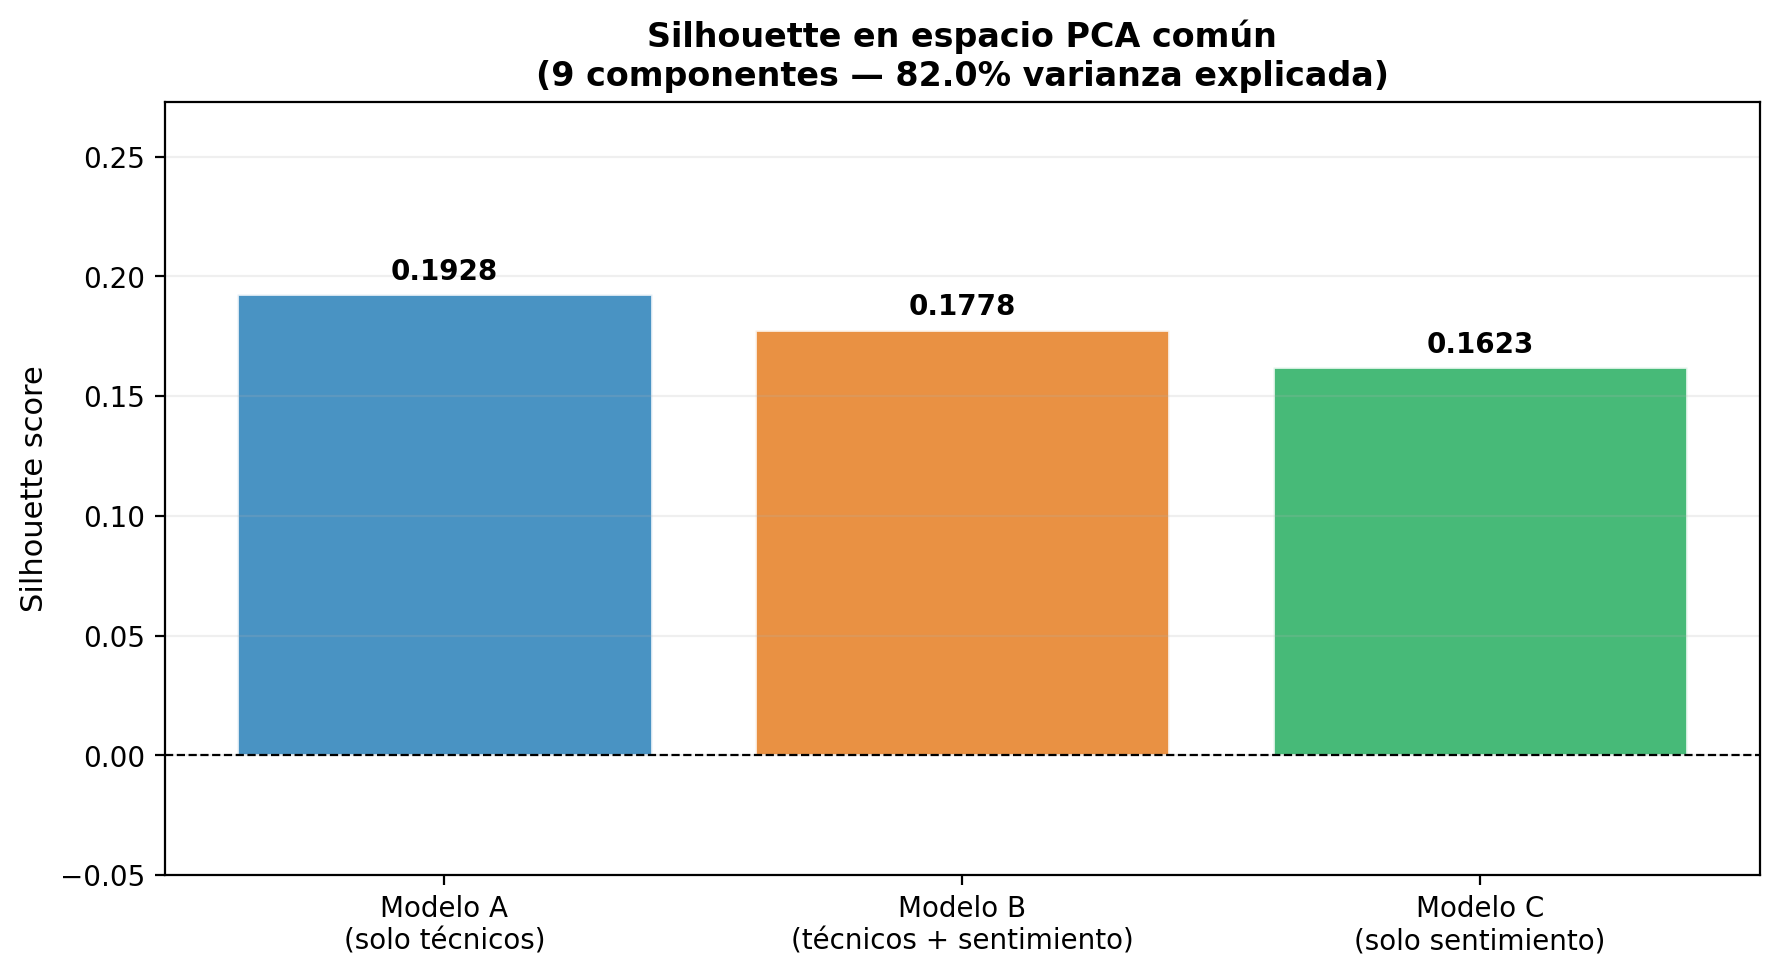
\includegraphics[width=0.85\textwidth]{figures/fig_silhouette_pca_comparison.png}
  \caption{Silhouette coefficient for Models A, B and C, computed in the common 9-component PCA space (82.0\% explained variance).}
  \label{fig:silhouette-pca-comparison}
\end{figure}

\begin{figure}[H]
  \centering
  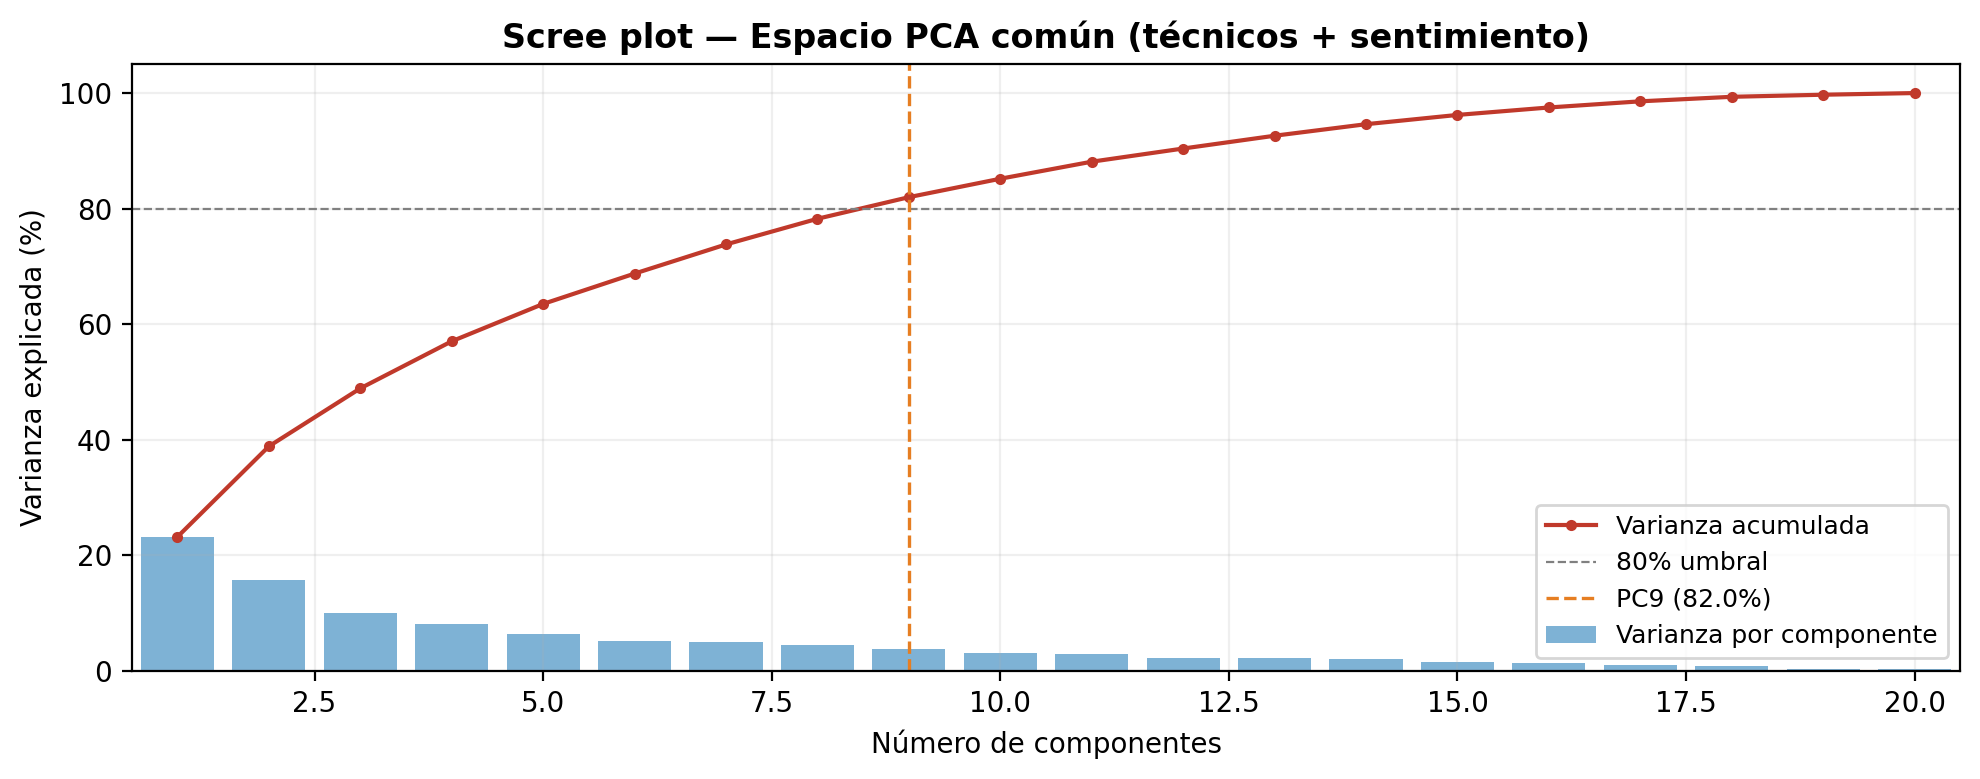
\includegraphics[width=0.85\textwidth]{figures/fig_silhouette_scree.png}
  \caption{Scree plot (cumulative explained variance) for the PCA decomposition of the 20-feature space (9 technical + 11 smoothed sentiment features) used to construct the common comparison space.}
  \label{fig:silhouette-scree}
\end{figure}

\section{PCA Visualizations}
\label{sec:results-pca}

To visualize the cluster structure in two dimensions,
\Cref{fig:pca-modelA} and \Cref{fig:pca-modelB} show, for Models A and B
respectively, a three-panel figure consisting of (i) a 2D scatter plot of
the first two principal components, colored by regime label
(\emph{Bull} in green, \emph{Bear} in red, \emph{Crisis} in orange,
following the color convention $\{0:\texttt{\#0D7A3E}, 1:\texttt{\#C0392B},
2:\texttt{\#E67E22}\}$), (ii) the loadings of the original features on the
first two principal components, and (iii) the cumulative explained
variance (scree plot).

For Model A, PCA is applied to the 9 standardized technical features:
PC1 explains 43.7\% of the variance and PC2 an additional 15.8\%
(59.5\% jointly), and 4 components are required to reach 80\% of the
total variance. For Model B, to obtain a visualization that remains
interpretable while still reflecting the sentiment dimension, PCA is
applied to the 20-feature space consisting of the 9 technical features
plus the 11 MA21-\emph{smoothed} sentiment features (rather than the full
31-feature raw space used for clustering itself): PC1 explains 23.2\% and
PC2 an additional 15.7\% (38.9\% jointly), with 9 components required to
reach 80\% of the variance --- consistent with the common PCA space used
in \Cref{sec:results-silhouette}.

\begin{figure}[H]
  \centering
  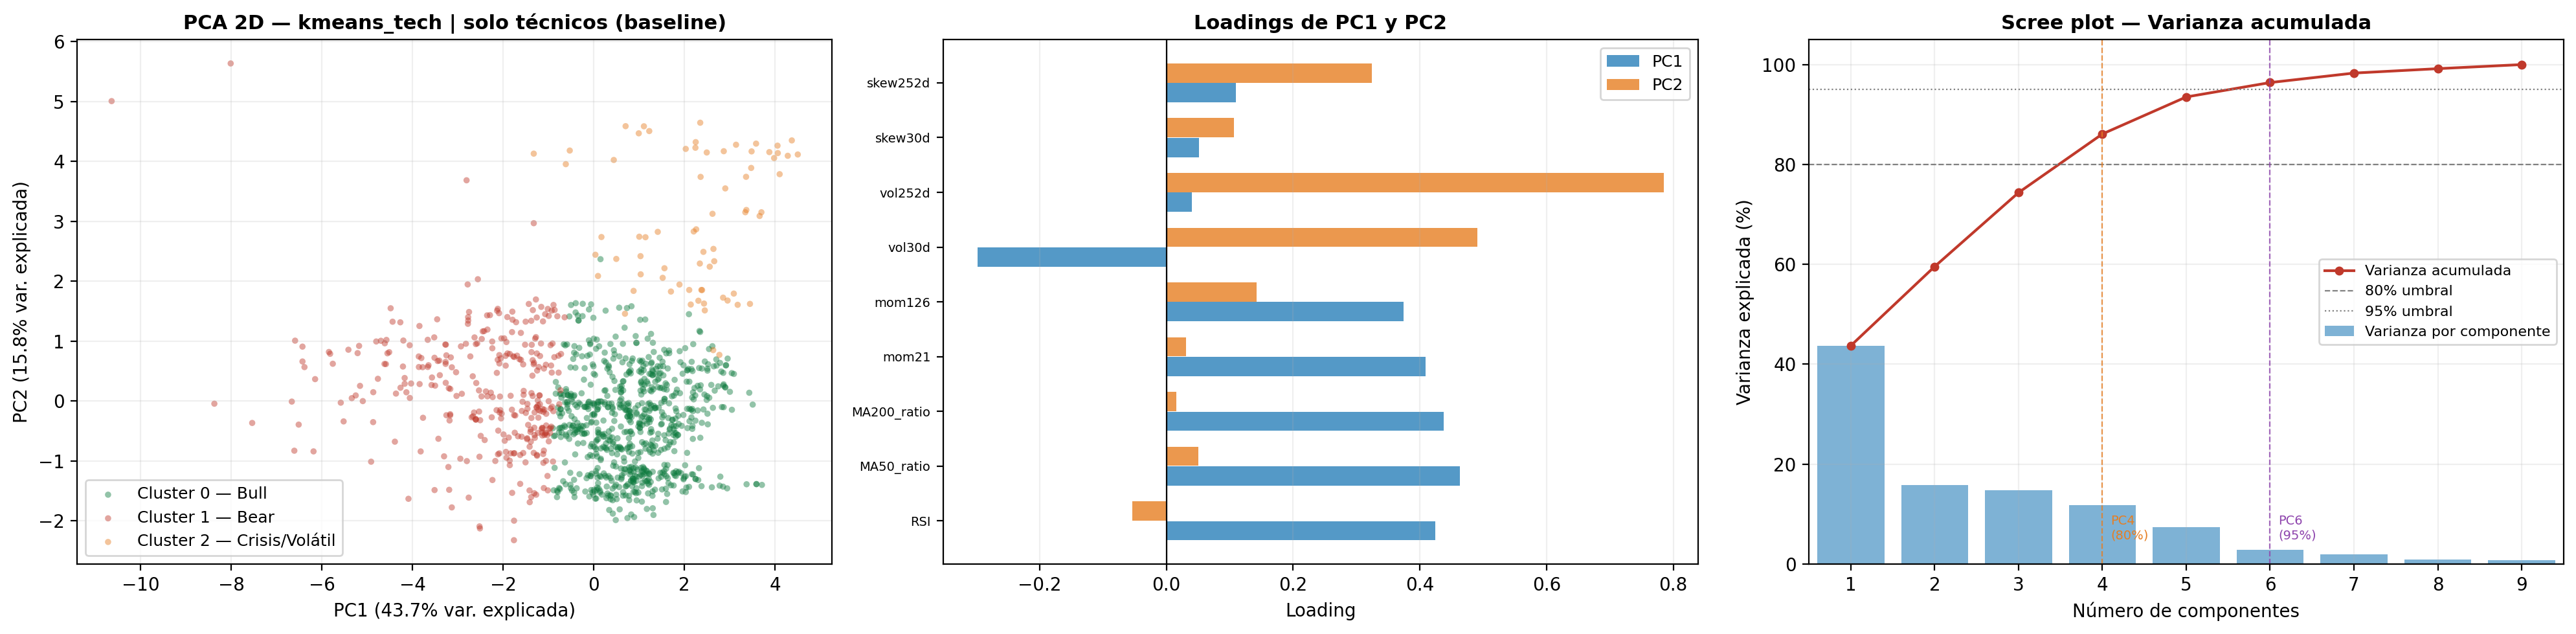
\includegraphics[width=\textwidth]{figures/fig_pca_modelA.png}
  \caption{Model A (technical only): PCA scatter plot of regimes (left), feature loadings on PC1/PC2 (center), and cumulative explained variance (right). PC1 (43.7\%) is dominated by volatility and RSI/momentum, separating the high-volatility \emph{Crisis} regime (orange) from the \emph{Bull} (green) and \emph{Bear} (red) regimes.}
  \label{fig:pca-modelA}
\end{figure}

\begin{figure}[H]
  \centering
  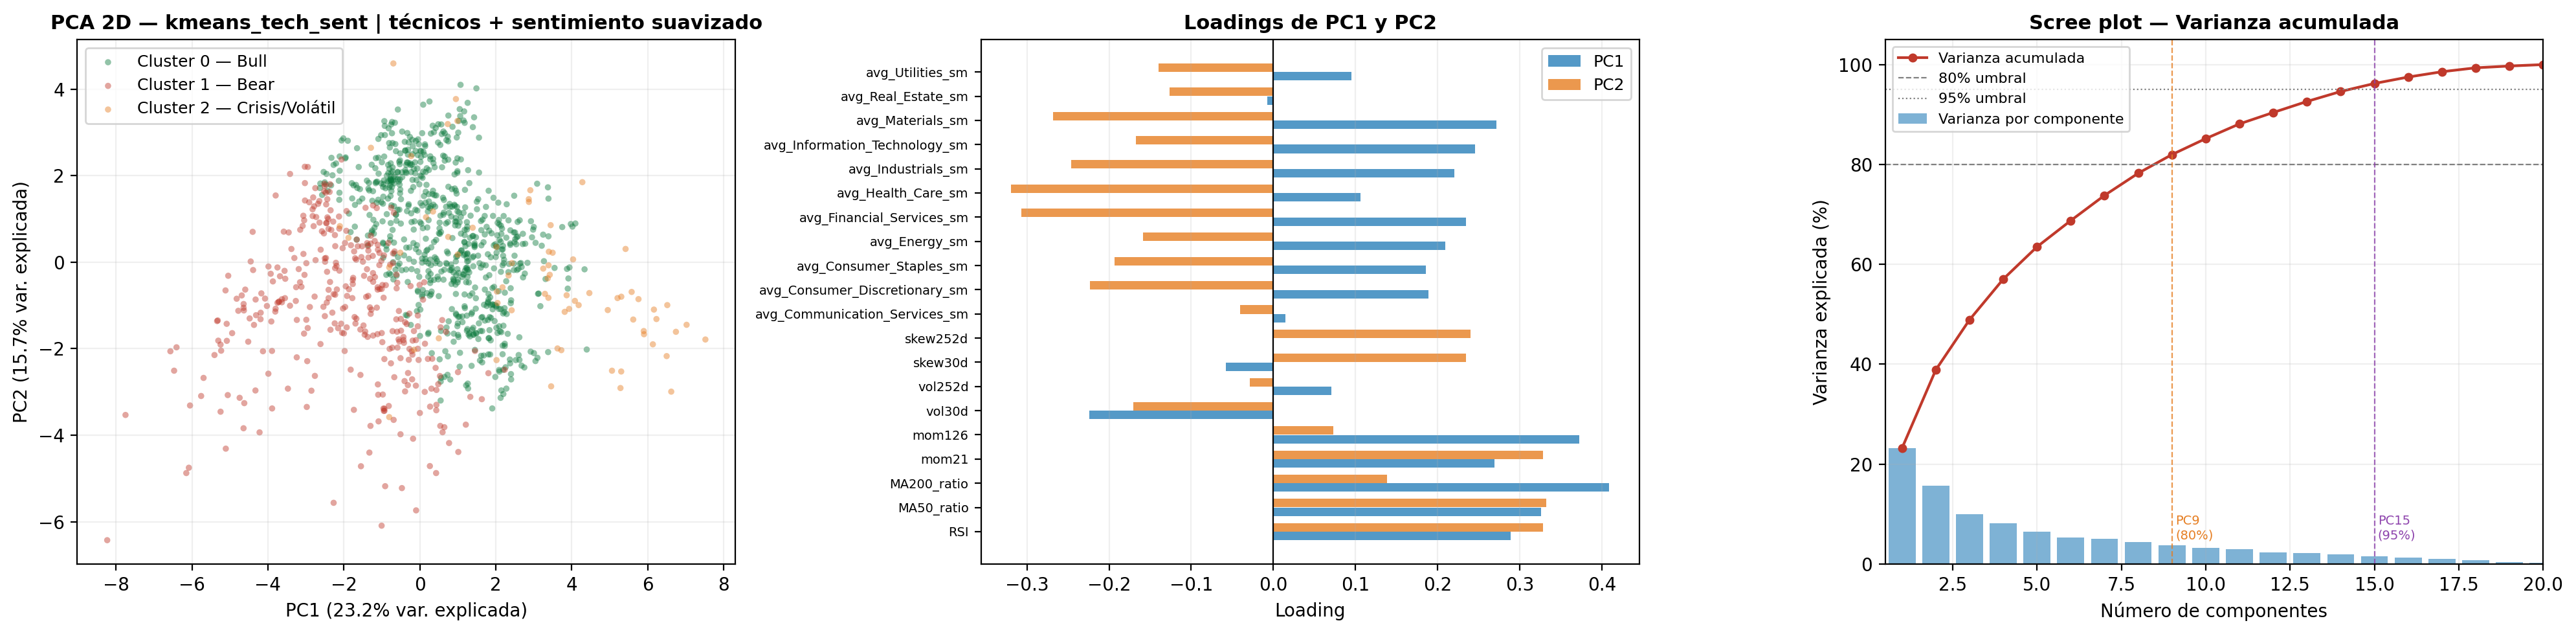
\includegraphics[width=\textwidth]{figures/fig_pca_modelB.png}
  \caption{Model B (technical + sentiment): PCA scatter plot of regimes (left; PCA computed on technical + MA21-smoothed sentiment features for visualization), feature loadings on PC1/PC2 (center), and cumulative explained variance (right).}
  \label{fig:pca-modelB}
\end{figure}

In both figures, the \emph{Crisis} regime (orange, $n=70$ in both Models A
and B) appears as a comparatively small, visually distinct cloud of
points located towards the high-volatility extreme of PC1, consistent
with its centroid profile (\Cref{tab:centroids-modelA,tab:centroids-modelB}):
substantially higher \texttt{vol252d\_sp500} than the other two regimes.
The \emph{Bull} (green) and \emph{Bear} (red) regimes show greater overlap
along PC2, reflecting the smaller relative differences in
\texttt{vol30d\_sp500} and \texttt{skew30d\_sp500} between these two
regimes compared to the gap to \emph{Crisis}.

\section{Correlation Analysis}
\label{sec:results-correlation}

\Cref{fig:correlation-modelA} and \Cref{fig:correlation-modelB} show the
pairwise Pearson correlation matrices of the input features for Models A
and B, respectively. For Model A, strong positive correlations are
observed between \texttt{MA50\_ratio\_sp500}, \texttt{MA200\_ratio\_sp500}
and \texttt{RSI\_sp500} (all three increase together during uptrends), and
between \texttt{vol30d\_sp500} and \texttt{vol252d\_sp500} (short- and
long-term volatility co-move, though not perfectly, allowing the model to
distinguish transient volatility spikes from sustained high-volatility
regimes).

\begin{figure}[H]
  \centering
  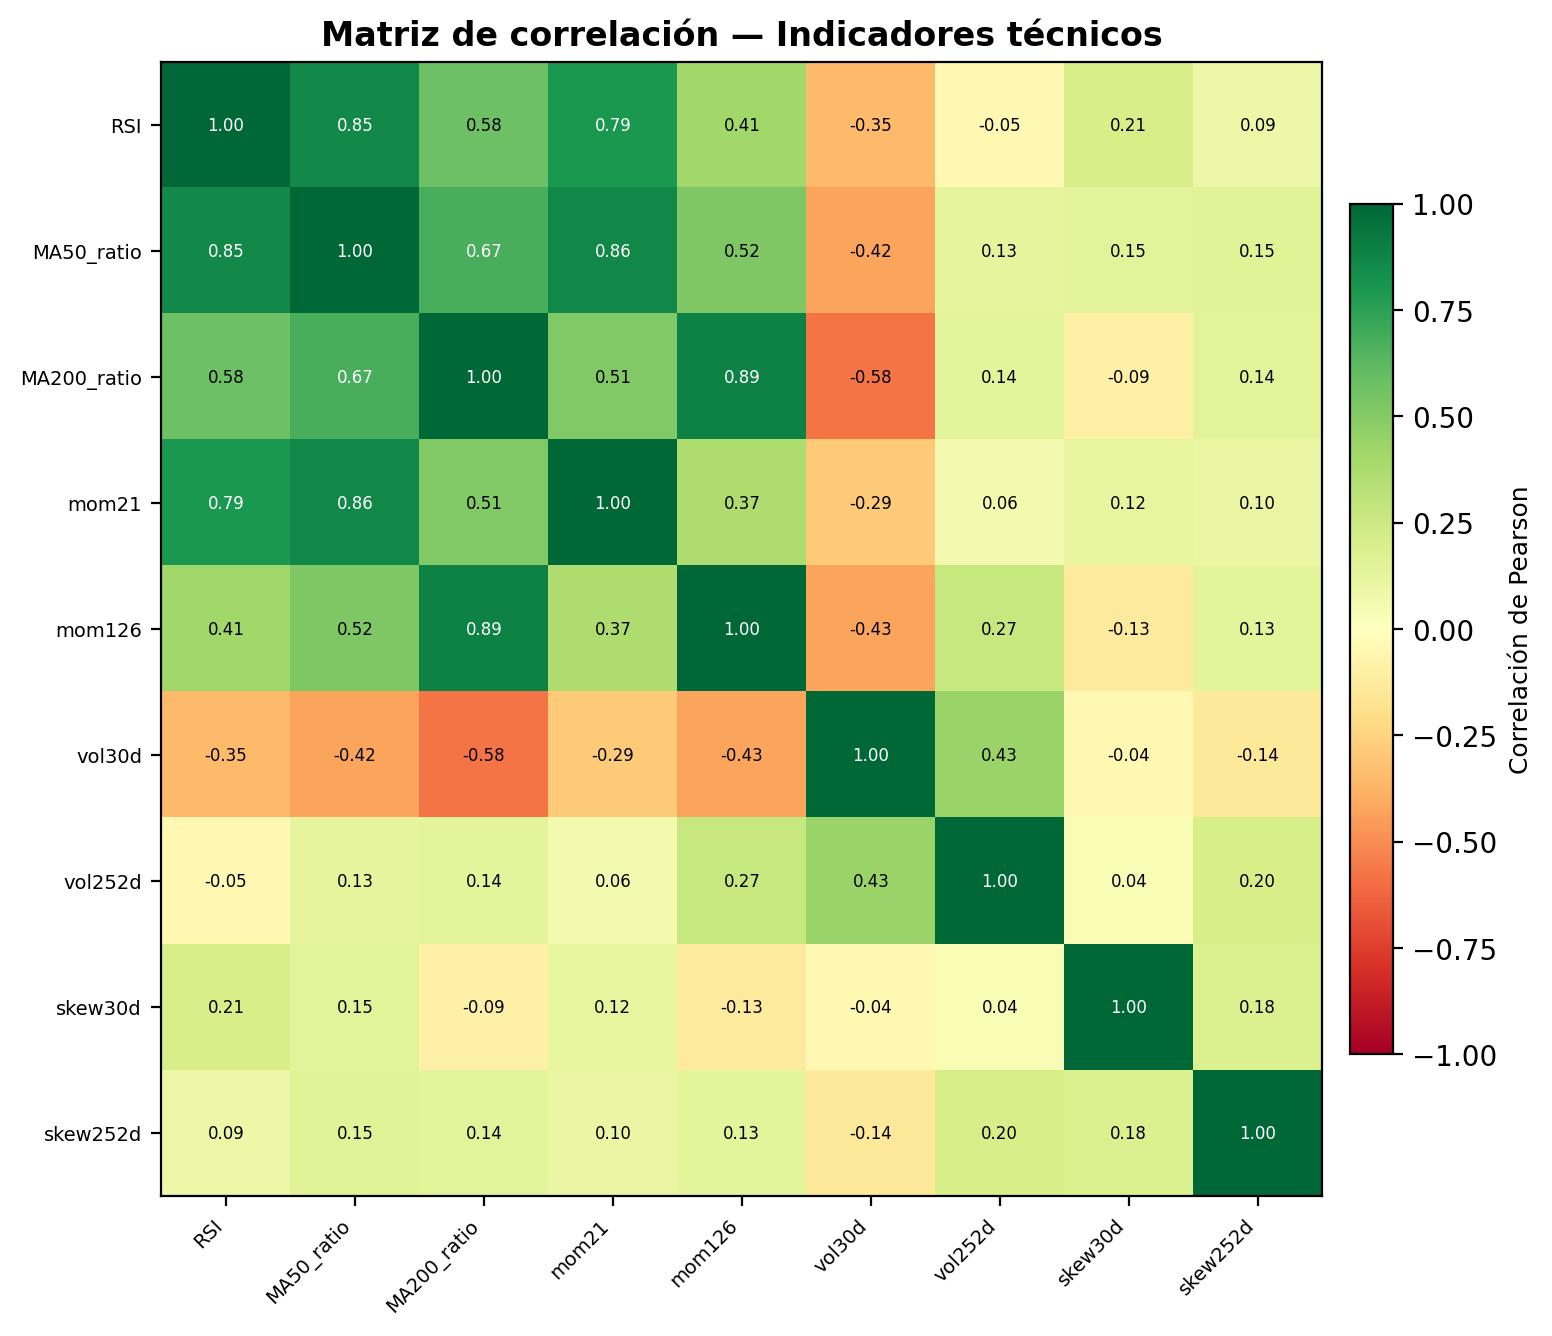
\includegraphics[width=0.85\textwidth]{figures/fig_correlation_modelA.png}
  \caption{Correlation matrix of the 9 technical features used in Model A.}
  \label{fig:correlation-modelA}
\end{figure}

For Model B, the correlation matrix additionally reveals the internal
structure of the 22 raw sentiment features. Two patterns are notable.
First, the \texttt{sentiment\_std\_<sector>} columns are strongly
positively correlated \emph{with each other} across sectors --- on days
with many news items across the market, sentiment dispersion tends to be
elevated simultaneously across most sectors, reflecting overall news
volume rather than sector-specific dynamics. Second, correlations between
sentiment features and technical features are generally \textbf{weak}
(typically below $|0.2|$), indicating that the sentiment signal captures
information that is largely \emph{orthogonal} to the price-derived
technical indicators --- a necessary (though not sufficient) condition for
sentiment to provide \emph{incremental} information to the clustering
model, rather than being redundant with the technical features already
present in Model A.

\begin{figure}[H]
  \centering
  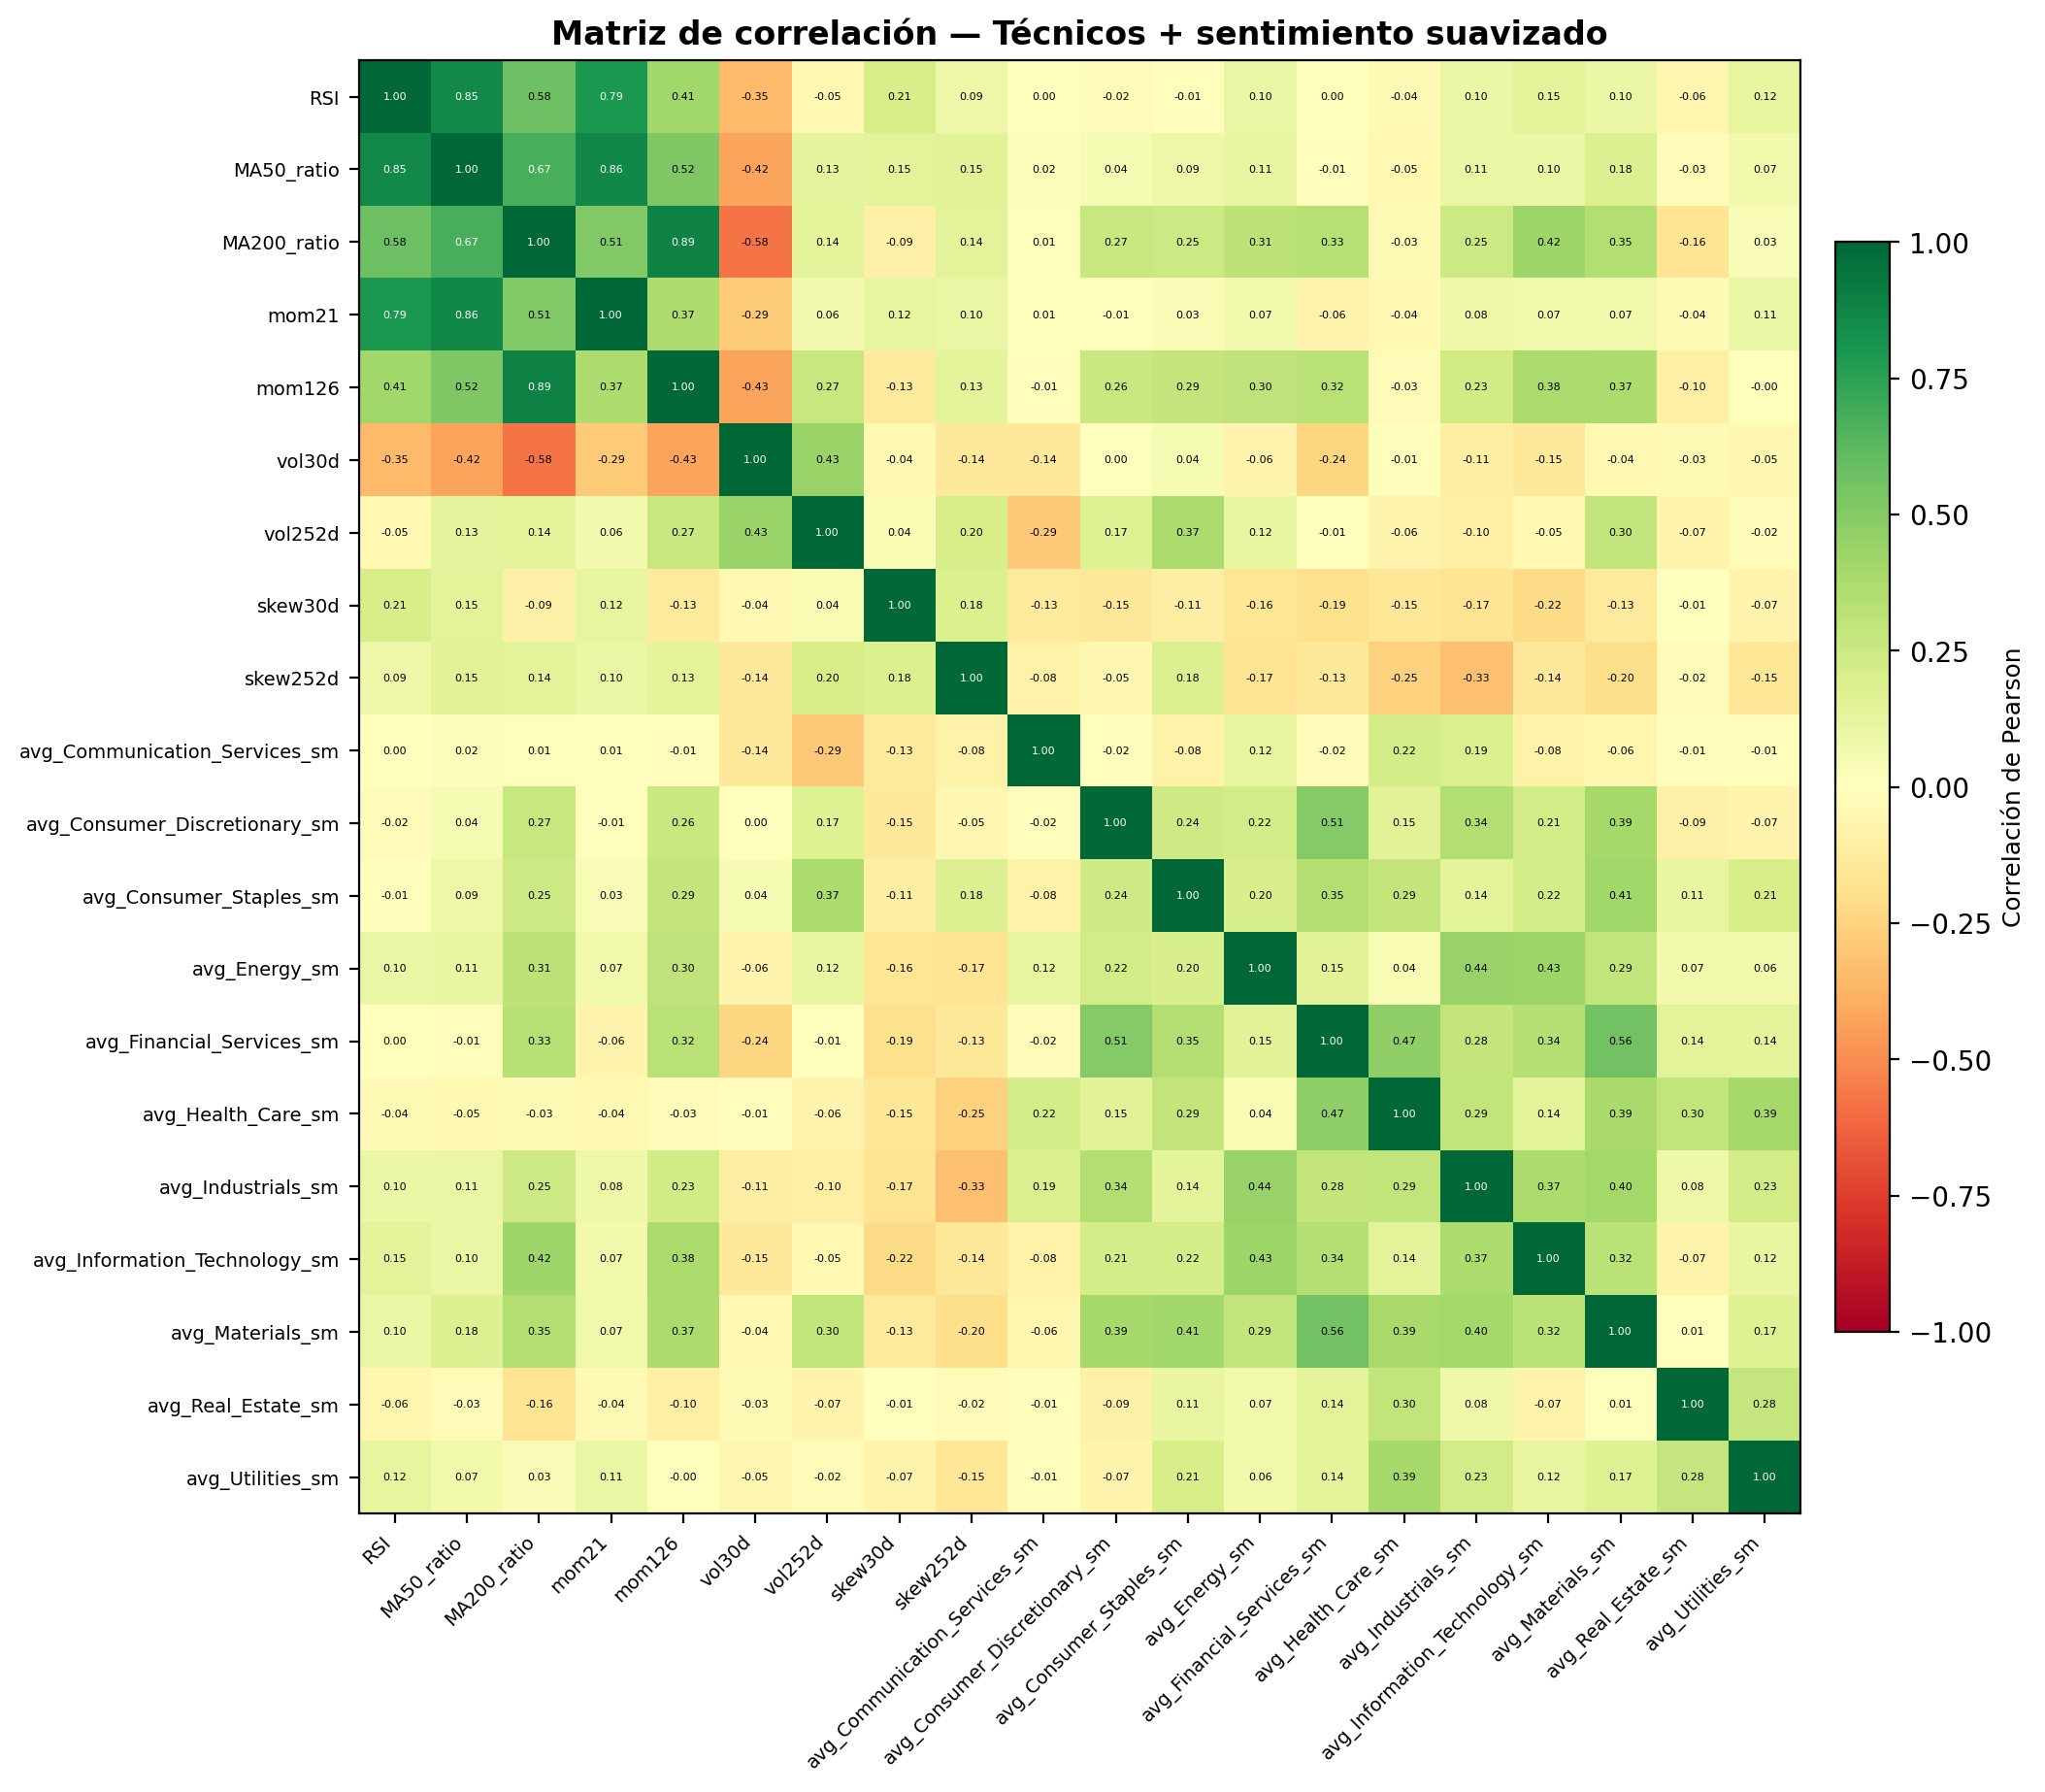
\includegraphics[width=0.95\textwidth]{figures/fig_correlation_modelB.png}
  \caption{Correlation matrix of the 31 features used in Model B (9 technical + 22 raw sector sentiment features).}
  \label{fig:correlation-modelB}
\end{figure}

\section{Feature Importance}
\label{sec:results-importance}

To assess which features contribute most to the partition produced by
Model B (\texttt{kmeans\_tech\_sent}), an ANOVA F-statistic is computed
for each feature, comparing its between-cluster variance to its
within-cluster variance: features with a large F-statistic vary
substantially \emph{across} the three regimes relative to how much they
vary \emph{within} each regime, and are therefore the features that most
strongly characterize the partition. \Cref{tab:feature-importance} reports
the top 10 features by F-statistic, and \Cref{fig:feature-importance}
shows the corresponding figure.

\begin{table}[H]
\centering
\caption{Top 10 features by ANOVA F-statistic for Model B (\texttt{kmeans\_tech\_sent}). All $p$-values are far below $10^{-50}$.}
\label{tab:feature-importance}
\small
\begin{tabular}{lllr}
\toprule
\textbf{Rank} & \textbf{Feature} & \textbf{Type} & \textbf{F-statistic} \\
\midrule
1  & MA50\_ratio\_sp500                    & Technical            & 597.81 \\
2  & RSI\_sp500                             & Technical            & 561.49 \\
3  & MA200\_ratio\_sp500                    & Technical            & 526.13 \\
4  & vol252d\_sp500                         & Technical            & 454.17 \\
5  & mom21\_sp500                           & Technical            & 366.92 \\
6  & mom126\_sp500                          & Technical            & 333.83 \\
7  & sentiment\_std\_Information Technology & Raw sentiment        & 307.21 \\
8  & sentiment\_std\_Consumer Staples       & Raw sentiment        & 295.60 \\
9  & sentiment\_std\_Consumer Discretionary & Raw sentiment        & 276.30 \\
10 & sentiment\_std\_Energy                 & Raw sentiment        & 267.58 \\
\bottomrule
\end{tabular}
\end{table}

\begin{figure}[H]
  \centering
  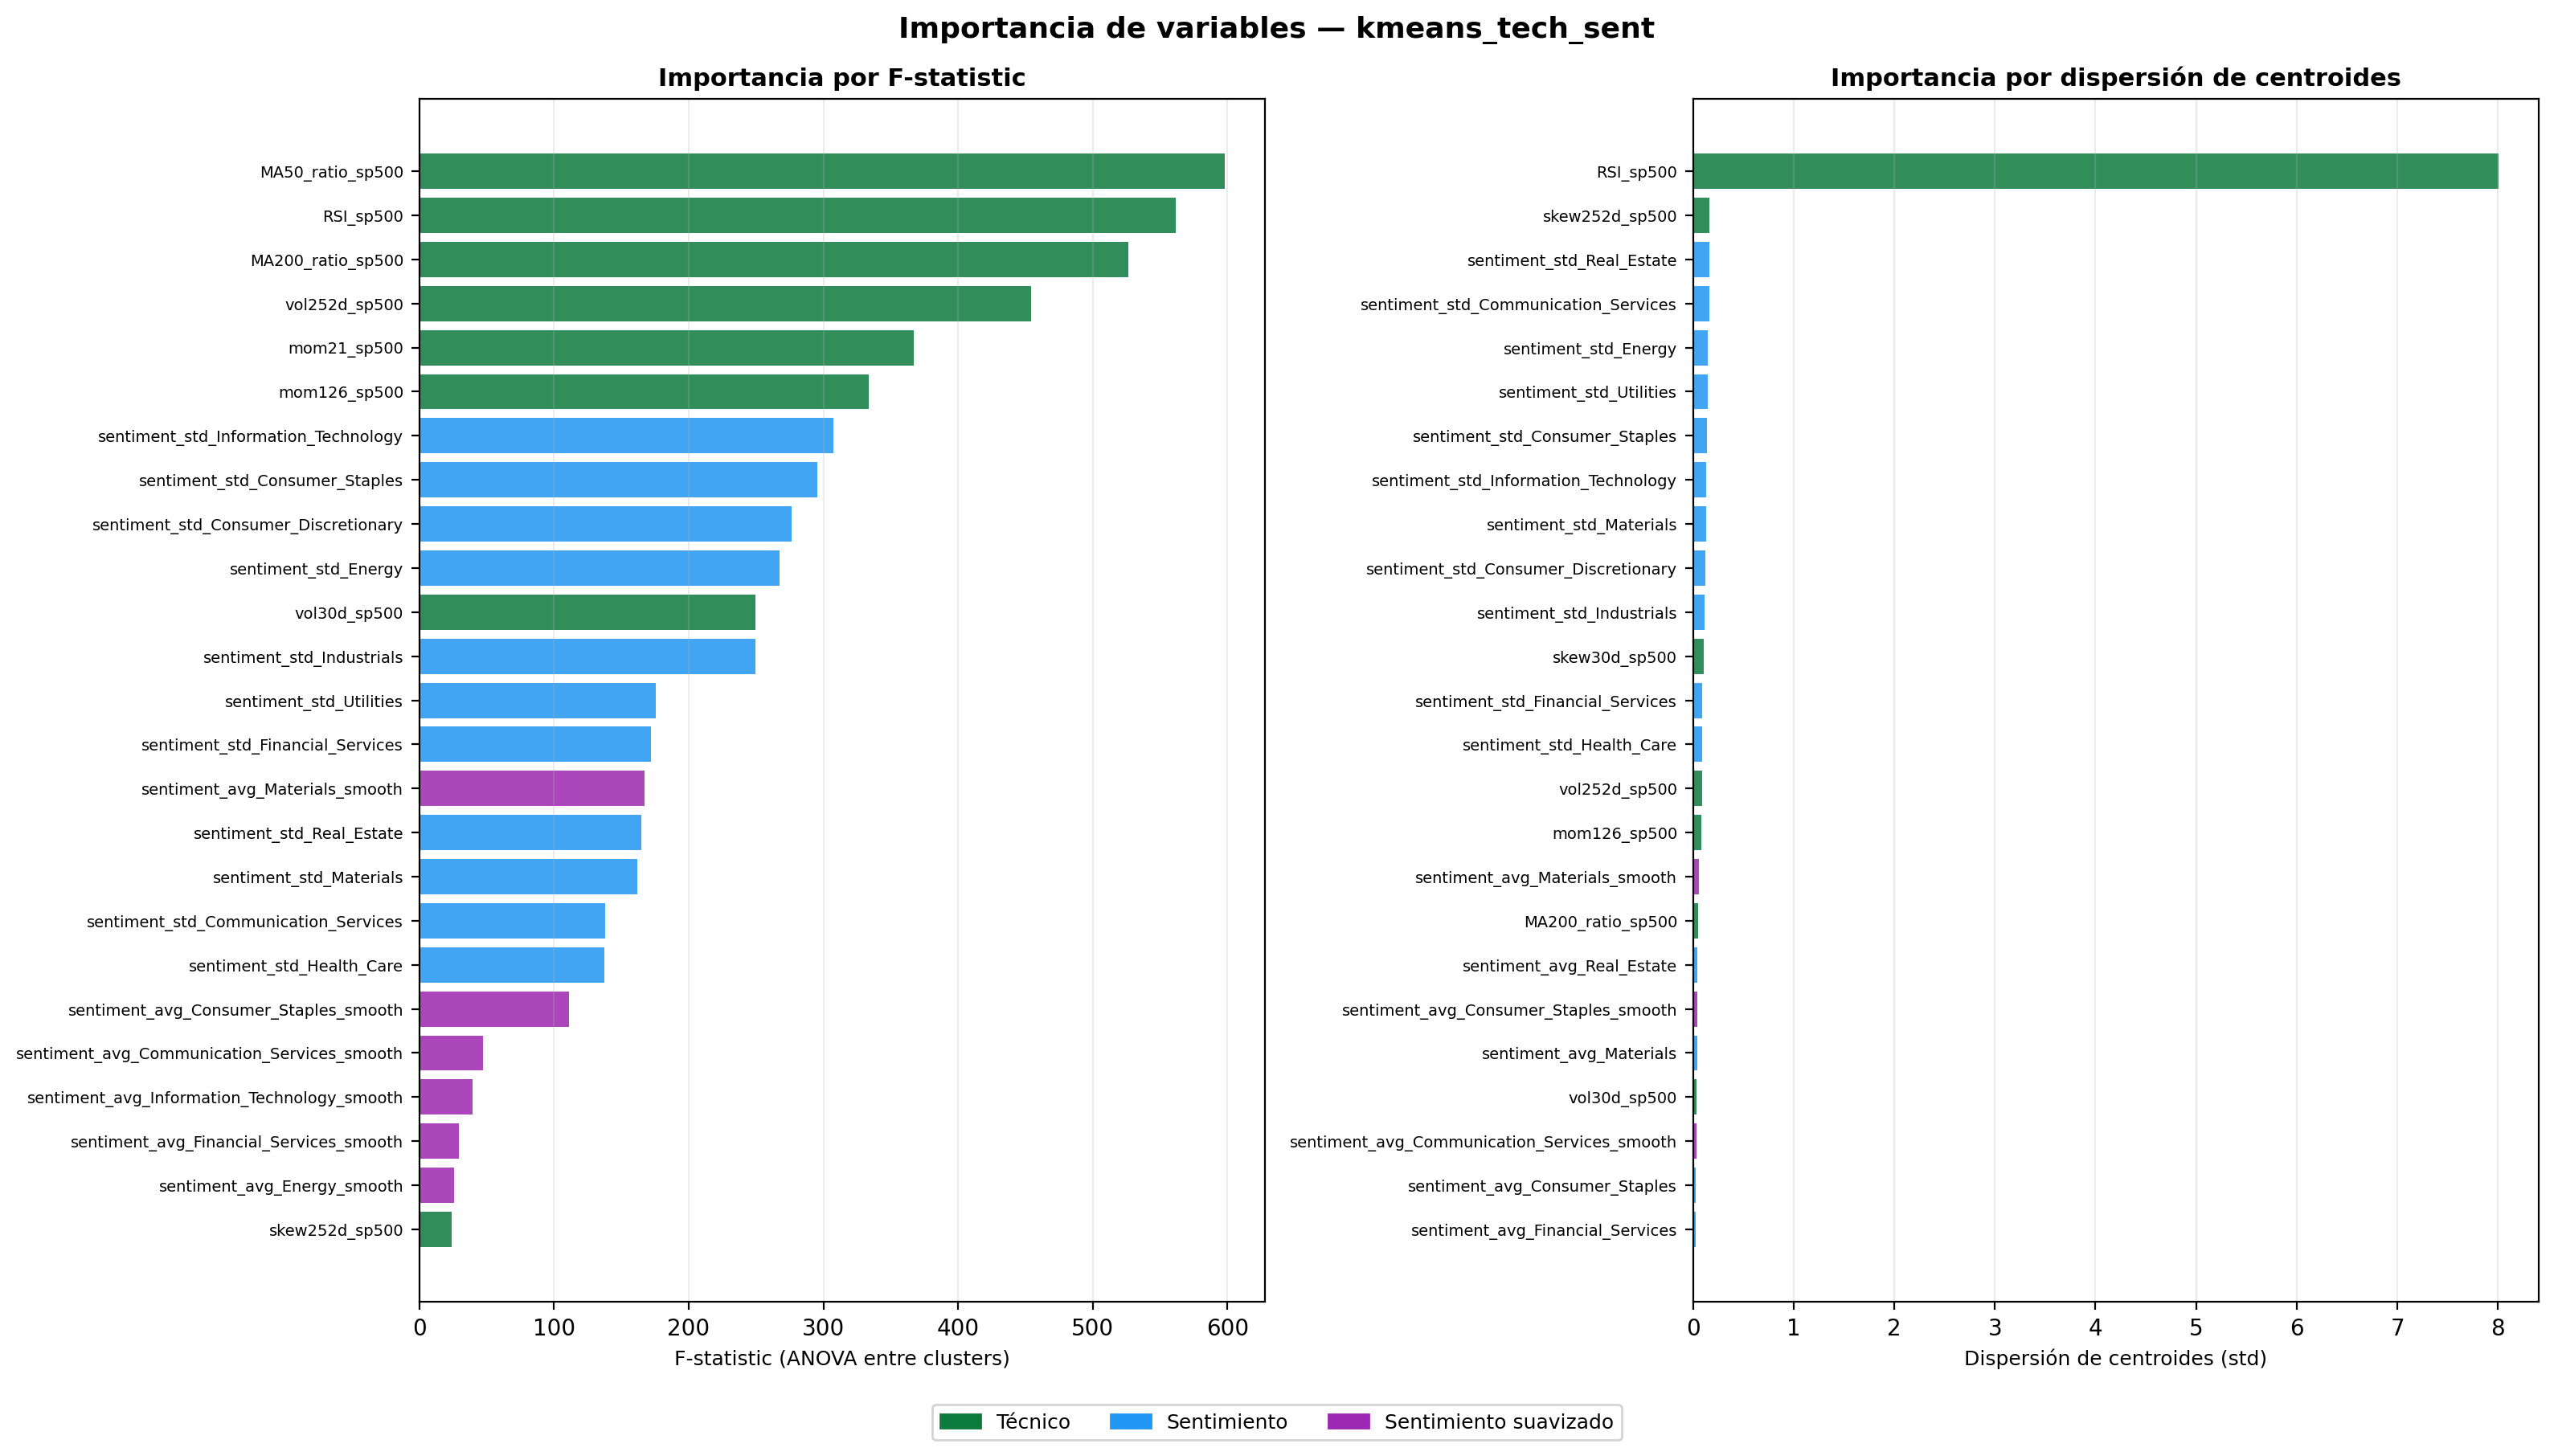
\includegraphics[width=0.95\textwidth]{figures/fig_feature_importance.png}
  \caption{ANOVA F-statistic by feature for Model B (\texttt{kmeans\_tech\_sent}), highlighting the dominance of technical features (RSI, moving-average ratios, volatility, momentum) but also the substantial contribution of sentiment-dispersion (\texttt{sentiment\_std}) features for several sectors.}
  \label{fig:feature-importance}
\end{figure}

The results in \Cref{tab:feature-importance} confirm the dominant role of
\emph{technical} features --- the top 6 features by F-statistic are all
technical indicators, with \texttt{MA50\_ratio\_sp500} ($F=597.81$) and
\texttt{RSI\_sp500} ($F=561.49$) leading. However, the \textbf{7th to
10th-ranked} features are all \texttt{sentiment\_std\_<sector>} columns
(\emph{Information Technology}, \emph{Consumer Staples}, \emph{Consumer
Discretionary} and \emph{Energy}), with F-statistics in the range
267--307 --- the same order of magnitude as \texttt{vol30d\_sp500}
($F=249.61$, ranked 11th). This indicates that the \emph{dispersion} of
sector sentiment (i.e., the degree of disagreement among simultaneous news
items about a sector) is, in fact, one of the more discriminative
sentiment-derived features for the Model B partition --- considerably more
so than the corresponding \texttt{sentiment\_avg\_<sector>} mean-sentiment
columns, all of which rank below position 20 (with F-statistics below 50).
This suggests that \emph{how much disagreement} there is in the news flow
about a sector is more informative for regime discrimination than the
\emph{average tone} of that news flow.

\section{Regime Distribution and Temporal Analysis}
\label{sec:results-regimes}

\Cref{fig:sp500-regimes-modelA} and \Cref{fig:sp500-regimes-modelB} plot
the S\&P 500 closing price over the full sample period, with the
background shaded according to the regime detected by Models A and B,
respectively (green = Bull, red = Bear, orange = Crisis). Both models
identify the \emph{Crisis} regime ($n=70$ days in both cases, 6.2\% of the
sample) almost exclusively around two episodes: the recovery phase
following the 2008--2009 financial crisis (2009) and the COVID-19 market
crash and rebound of early-to-mid 2020 --- both periods characterized by
the combination of extreme realized volatility and strong 126-session
momentum (a sharp V-shaped recovery) that defines the \emph{Crisis}
centroid in \Cref{tab:centroids-modelA,tab:centroids-modelB}.

\begin{figure}[H]
  \centering
  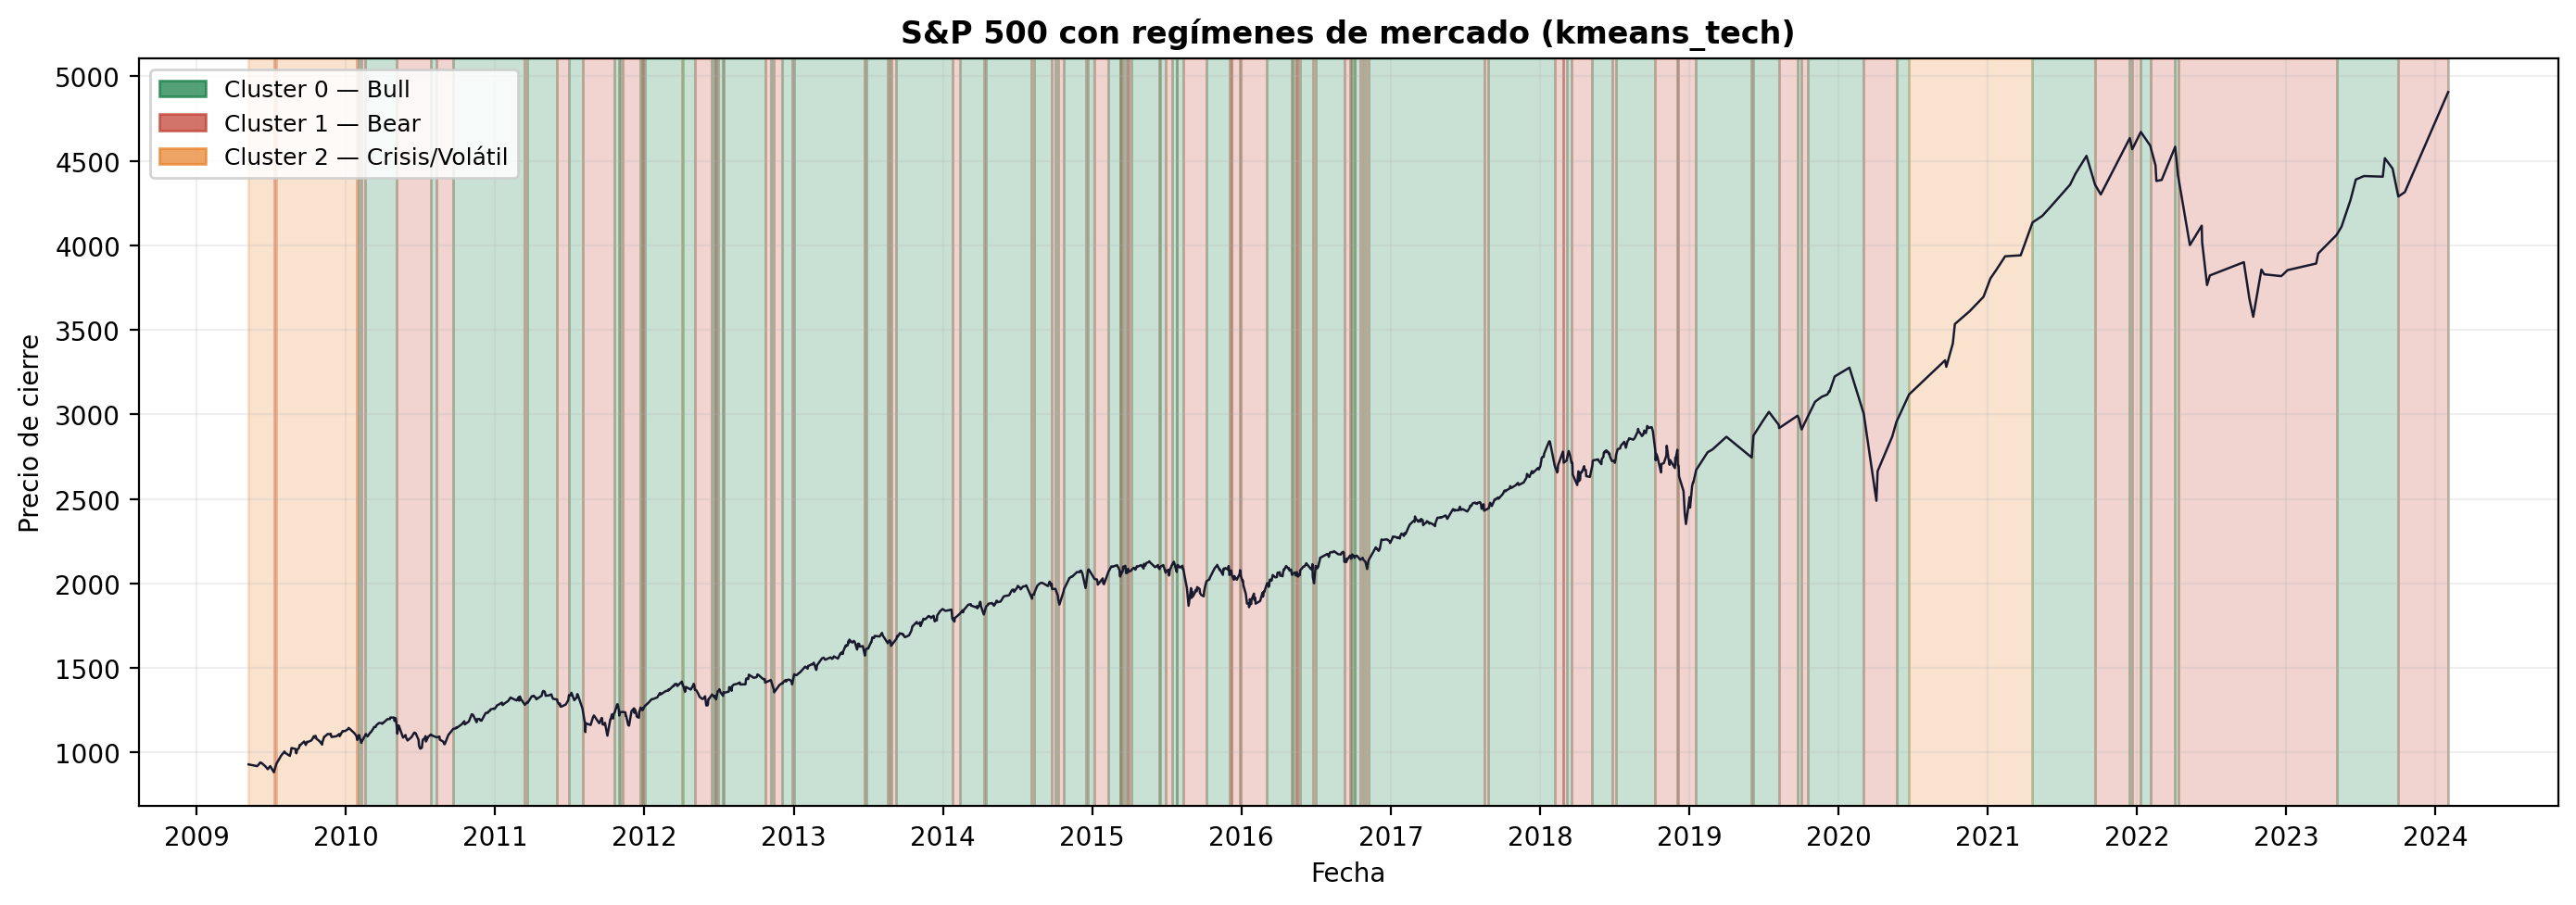
\includegraphics[width=\textwidth]{figures/fig_sp500_regimes_modelA.png}
  \caption{S\&P 500 closing price with background shading by Model A regime (\texttt{kmeans\_tech}): green = Bull, red = Bear, orange = Crisis.}
  \label{fig:sp500-regimes-modelA}
\end{figure}

\begin{figure}[H]
  \centering
  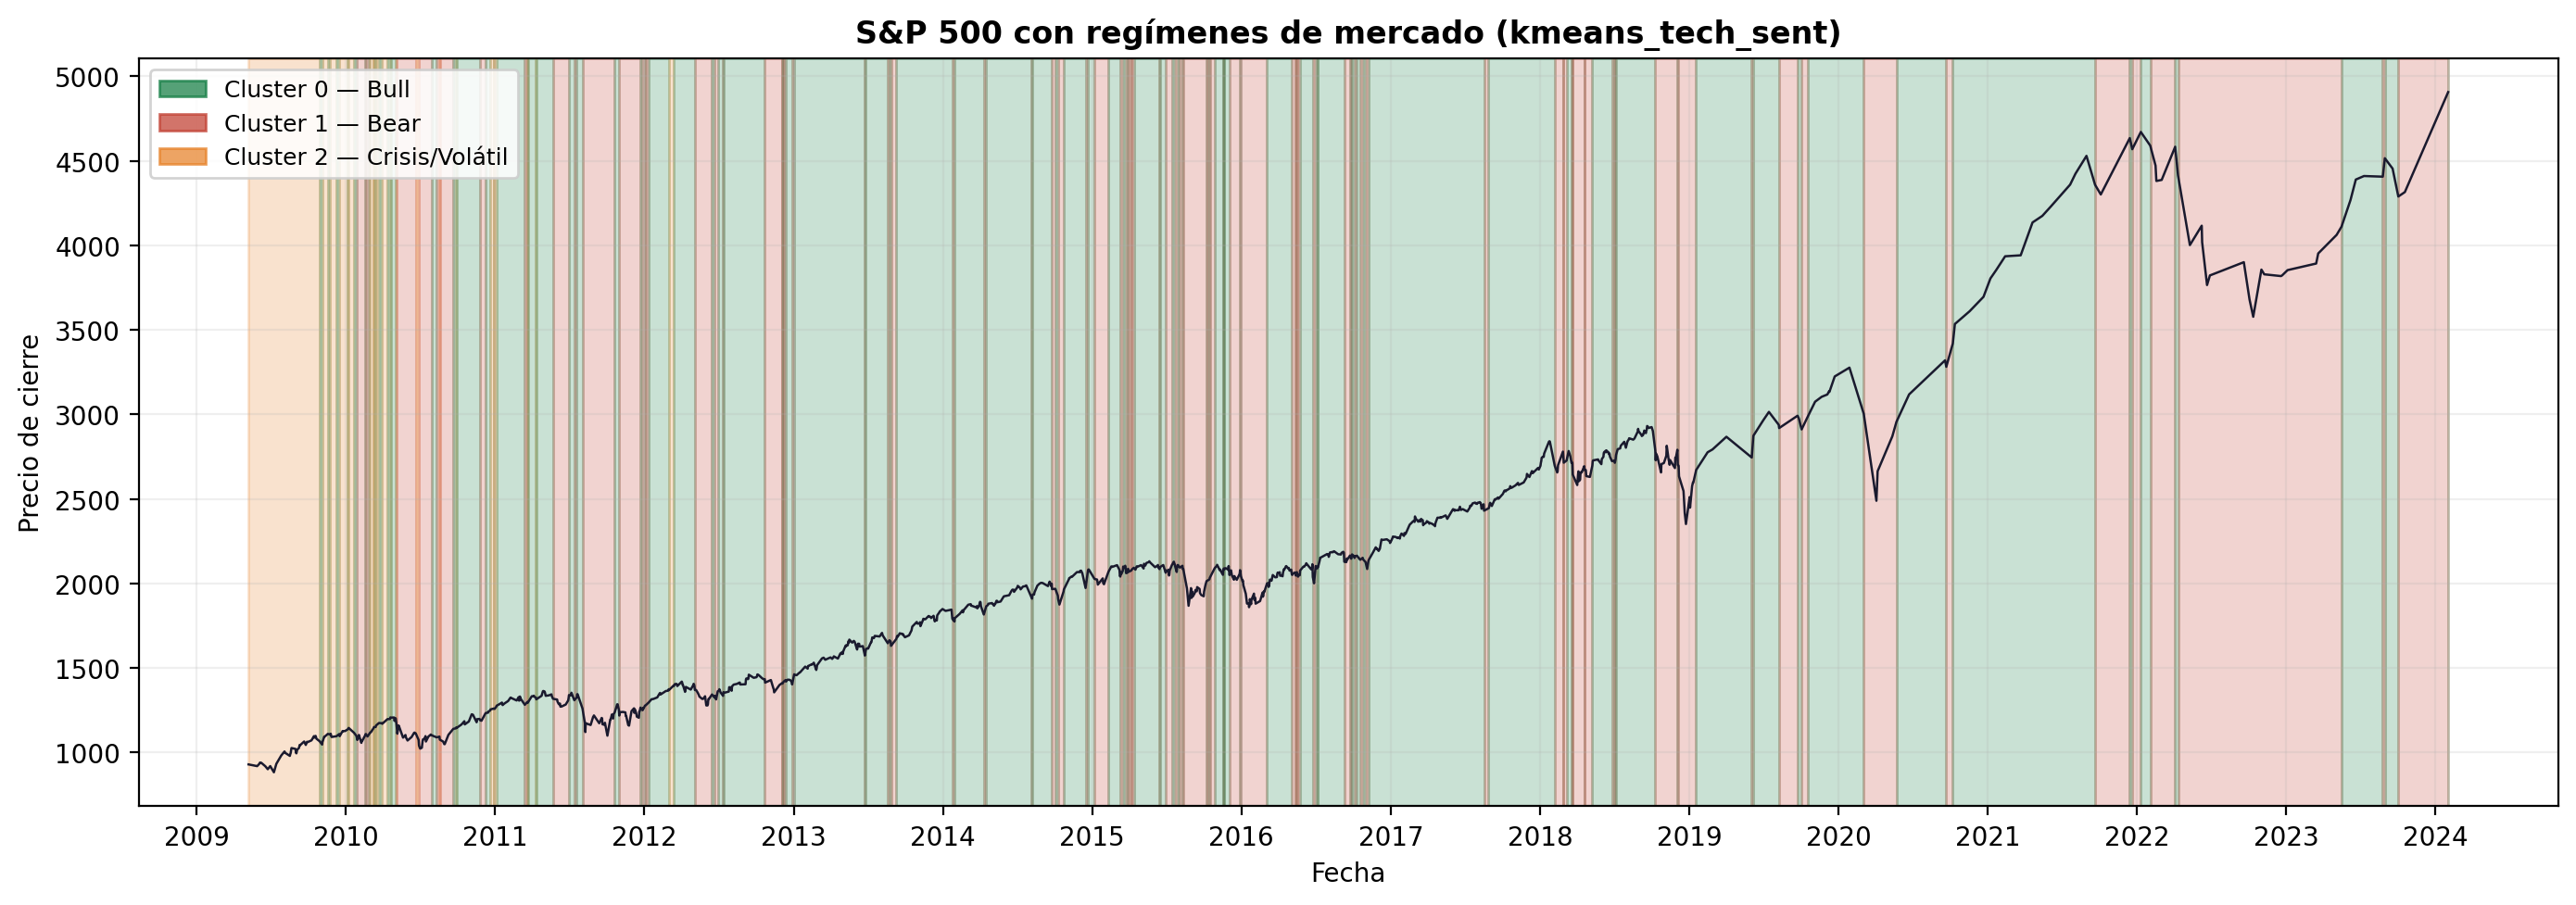
\includegraphics[width=\textwidth]{figures/fig_sp500_regimes_modelB.png}
  \caption{S\&P 500 closing price with background shading by Model B regime (\texttt{kmeans\_tech\_sent}): green = Bull, red = Bear, orange = Crisis.}
  \label{fig:sp500-regimes-modelB}
\end{figure}

The \emph{Bear} regime ($n=317$ for Model A, 28.0\%; $n=342$ for Model B,
30.2\%) is distributed across several multi-month episodes throughout the
sample, including parts of 2011 (European sovereign debt crisis), late
2015--early 2016, late 2018, and 2022. The \emph{Bull} regime is, in both
models, the majority class (65.8\% for Model A, 63.6\% for Model B),
reflecting the fact that the S\&P 500 spent the majority of the 2009--2024
sample in a long secular uptrend. The slightly larger \emph{Bear} share
and slightly smaller \emph{Bull} share in Model B relative to Model A
(and the corresponding 25-day reclassification of observations between the
two regimes, comparing $745\to720$ for Bull and $317\to342$ for Bear, with
\emph{Crisis} unchanged at $70$) indicates that incorporating sentiment
information causes a modest number of days that Model A classifies as
\emph{Bull} to be reclassified as \emph{Bear} by Model B --- consistent
with sentiment information being able to flag emerging weakness slightly
earlier or more persistently than technical indicators alone.

\Cref{fig:hmm-states-modelA} and \Cref{fig:hmm-states-modelB} show the
analogous state sequences produced by the Gaussian HMM (plotted as
\texttt{vol30d\_sp500} colored by HMM state over time, as produced by the
pipeline), which are discussed jointly with the economic comparison in
\Cref{sec:results-hmm}.

\begin{figure}[H]
  \centering
  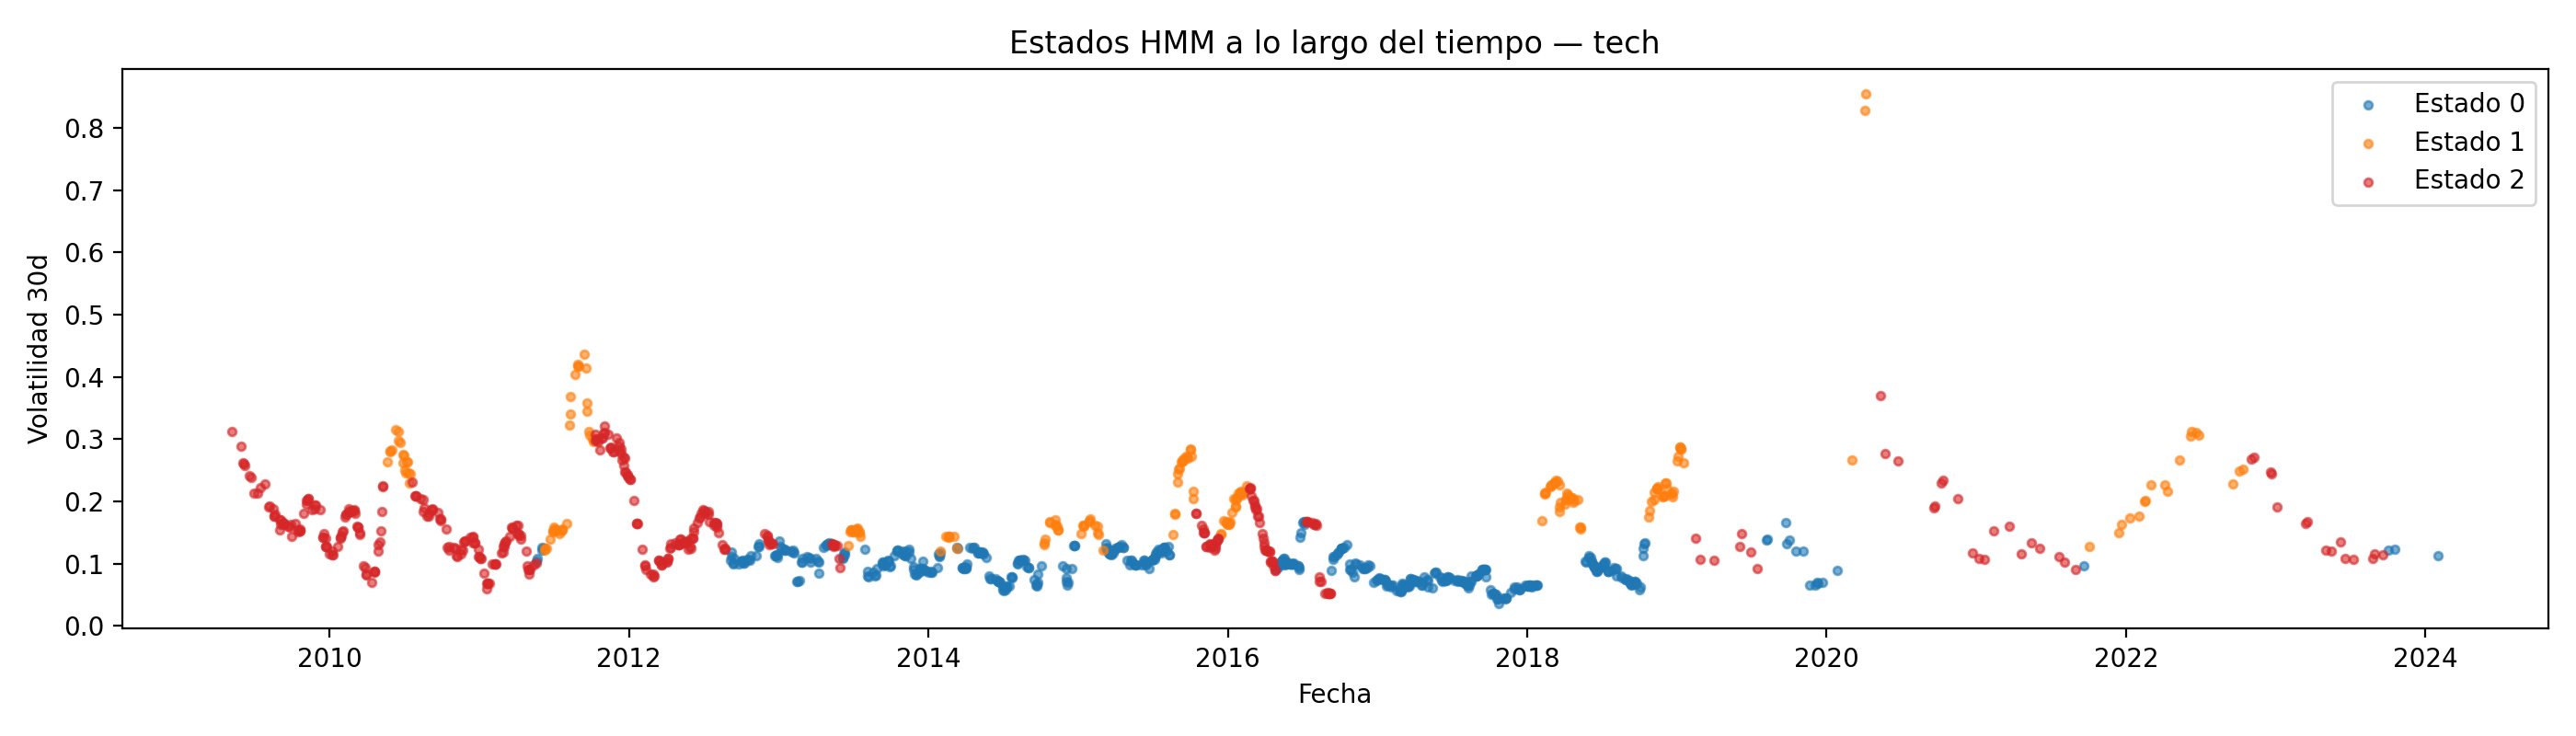
\includegraphics[width=\textwidth]{figures/fig_hmm_states_modelA.png}
  \caption{30-day realized volatility of the S\&P 500 over time, colored by Gaussian HMM state (\texttt{hmm\_tech}, fitted on the 9 technical features).}
  \label{fig:hmm-states-modelA}
\end{figure}

\begin{figure}[H]
  \centering
  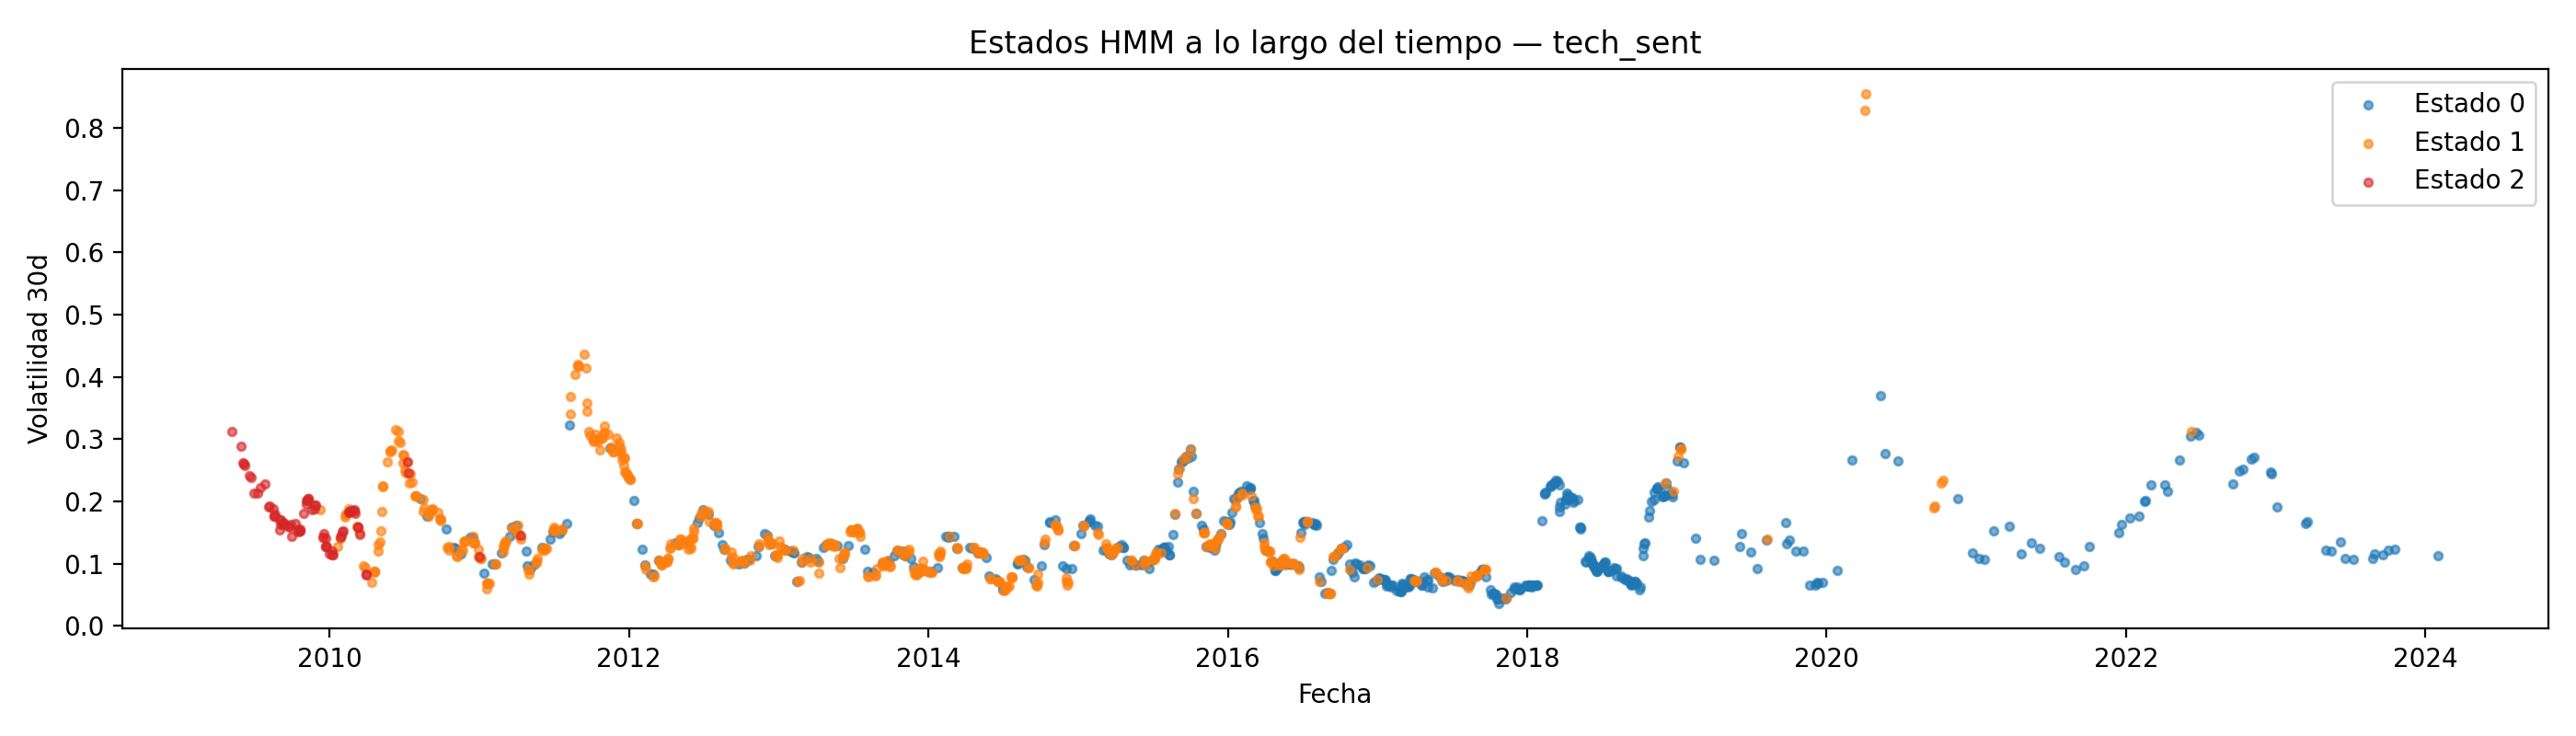
\includegraphics[width=\textwidth]{figures/fig_hmm_states_modelB.png}
  \caption{30-day realized volatility of the S\&P 500 over time, colored by Gaussian HMM state (\texttt{hmm\_tech\_sent}, fitted on the 31 technical + raw sentiment features).}
  \label{fig:hmm-states-modelB}
\end{figure}

\Cref{fig:sp500-regimes-hmm} shows the same regime-shading representation
as \Cref{fig:sp500-regimes-modelA,fig:sp500-regimes-modelB}, but for the
\texttt{hmm\_tech\_sent} state sequence. Visually, the HMM's \emph{Bear}
state (red) occupies a substantially larger fraction of the timeline than
the \textit{K-Means} \emph{Bear} regime, including extended stretches of
2011--2012, 2015--2016, 2018, 2020 and 2022 that \textit{K-Means} instead
assigns predominantly to \emph{Bull}. This is consistent with the
narrower, less extreme Sharpe ratios reported for the HMM in
\Cref{tab:market-hmm}: a \emph{Bear} state that includes a much larger and
more heterogeneous set of days necessarily has a less negative average
return than a \emph{Bear} regime restricted to the sharpest downturns.

\begin{figure}[H]
  \centering
  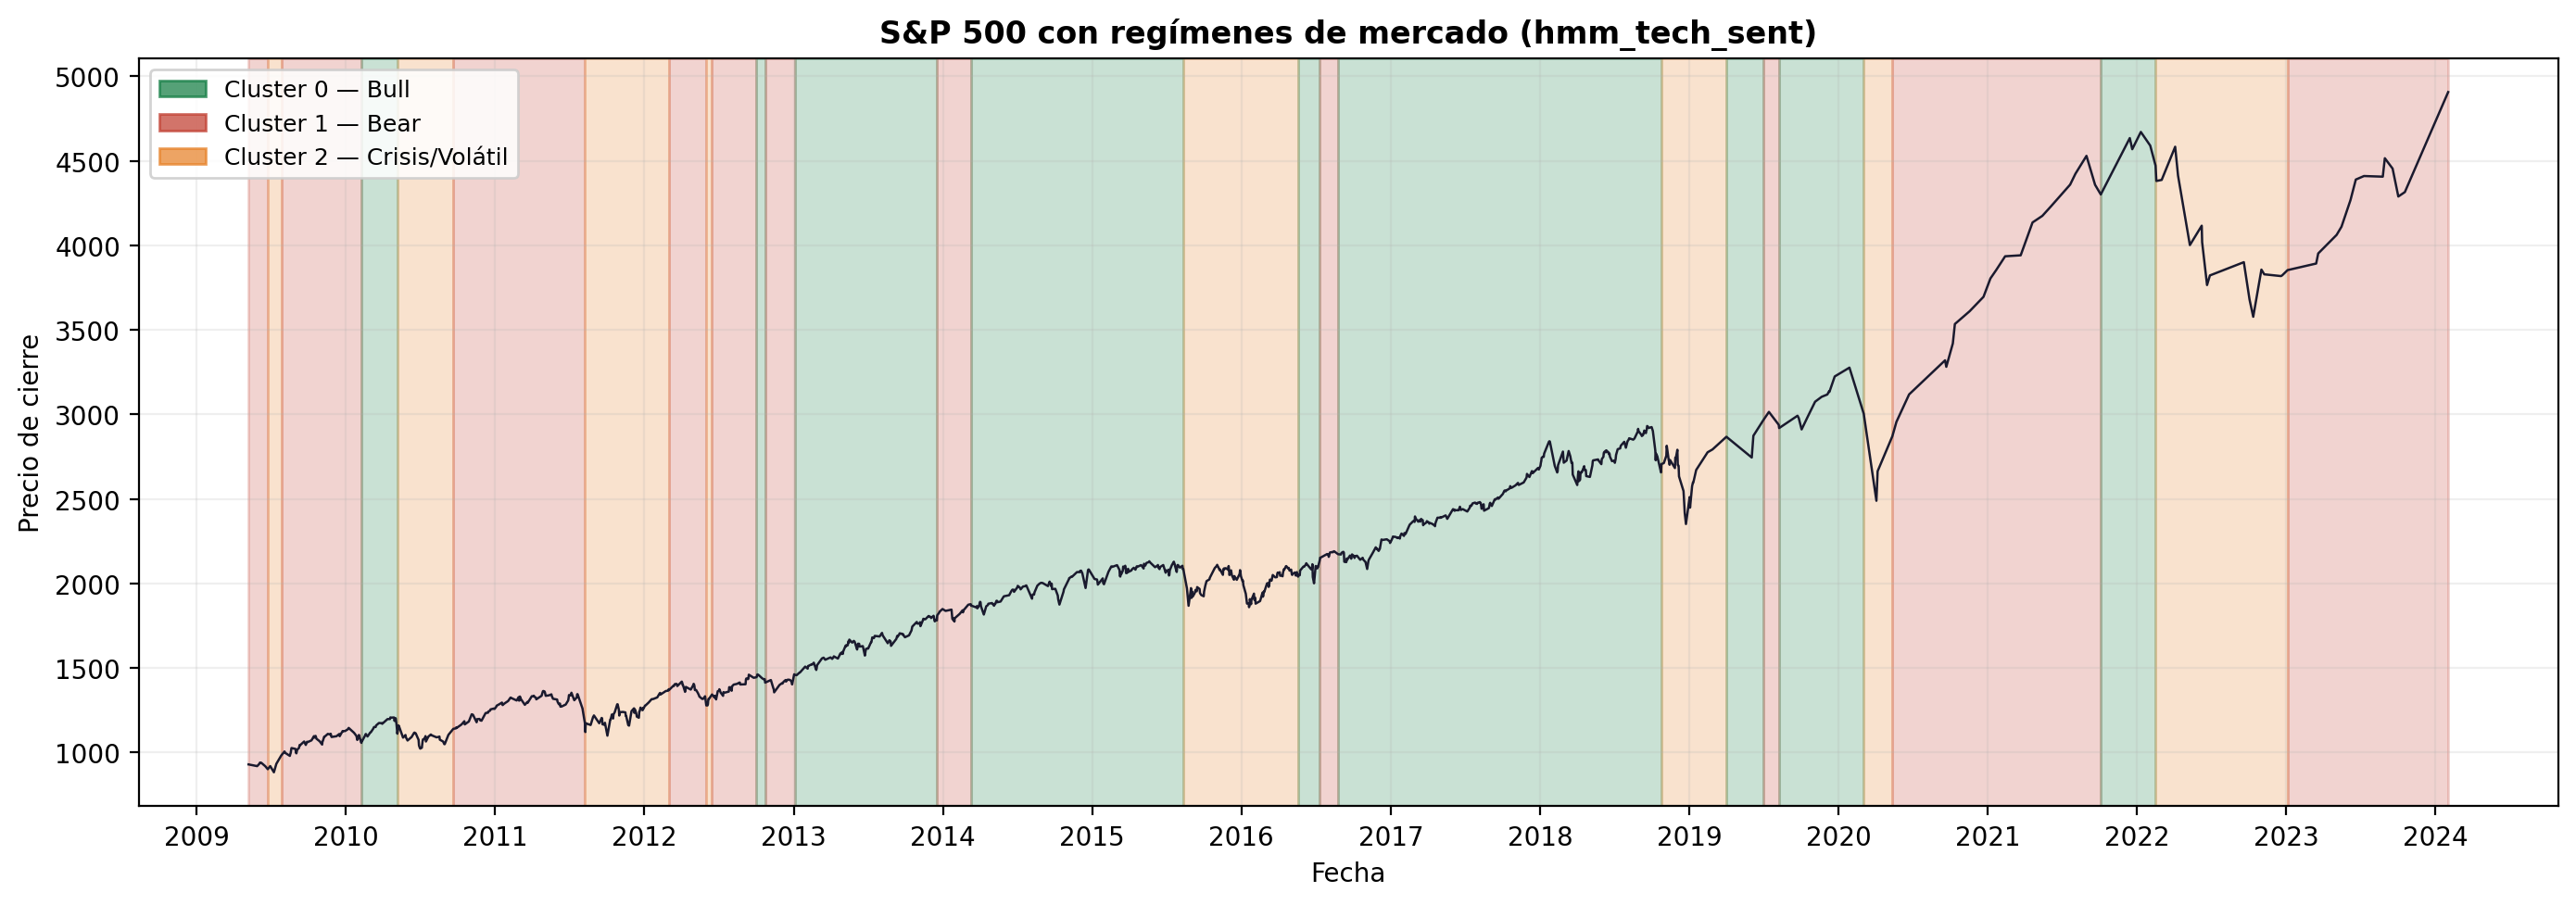
\includegraphics[width=\textwidth]{figures/fig_sp500_regimes_hmm.png}
  \caption{S\&P 500 closing price with background shading by Gaussian HMM state (\texttt{hmm\_tech\_sent}): green = Bull, red = Bear, orange = Crisis/Volatile.}
  \label{fig:sp500-regimes-hmm}
\end{figure}

\section{Economic Validation: Overall Market-Level Metrics}
\label{sec:results-econ-overall}

Before turning to the sector-level breakdown, this section reports the
economic profile of each regime computed directly on the \emph{aggregate}
S\&P 500 daily returns (i.e., not yet broken down by GICS sector), for all
five clustering configurations: Models A, B, C (\textit{K-Means}) and the
two HMM variants (\texttt{hmm\_tech}, \texttt{hmm\_tech\_sent}).
\Cref{tab:market-kmeans} and \Cref{tab:market-hmm} report, for each
regime/state, the number of days, the mean daily return, the annualized
volatility, the Sharpe ratio, the percentage of positive days, and the
best/worst single-day returns.

\begin{table}[H]
\centering
\caption{Market-level (S\&P 500) economic profile by regime, K-Means Models A, B and C. $n=1{,}132$ observations per model.}
\label{tab:market-kmeans}
\small
\begin{tabular}{llrrrrrr}
\toprule
\textbf{Model} & \textbf{Regime} & \textbf{$n$} & \textbf{Mean daily ret.\ (\%)} & \textbf{Ann.\ vol.} & \textbf{Sharpe} & \textbf{\% pos.\ days} & \textbf{Worst / Best day (\%)} \\
\midrule
A & Bull    & 745 & 0.1565  & 0.1018 & 3.68  & 59.7 & $-2.50$ / $3.37$ \\
A & Bear    & 317 & $-$0.2830 & 0.2352 & $-3.12$ & 41.6 & $-4.52$ / $6.80$ \\
A & Crisis  & 70  & 0.2315  & 0.1720 & 3.28  & 60.0 & $-2.46$ / $2.92$ \\
\midrule
B & Bull    & 720 & 0.1650  & 0.1035 & 3.82  & 60.0 & $-2.50$ / $3.37$ \\
B & Bear    & 342 & $-$0.2700 & 0.2289 & $-3.06$ & 42.1 & $-4.52$ / $6.80$ \\
B & Crisis  & 70  & 0.2369  & 0.1537 & 3.75  & 61.4 & $-2.46$ / $2.92$ \\
\midrule
C & Bull    & 534 & 0.0643  & 0.1711 & 0.83  & 53.9 & $-4.52$ / $4.63$ \\
C & Bear    & 172 & 0.1012  & 0.1386 & 1.70  & 58.7 & $-2.11$ / $2.92$ \\
C & Crisis  & 426 & $-$0.0204 & 0.1490 & $-0.48$ & 54.0 & $-3.34$ / $6.80$ \\
\bottomrule
\end{tabular}
\end{table}

\begin{table}[H]
\centering
\caption{Market-level (S\&P 500) economic profile by state, Gaussian HMM fitted on Model A and Model B feature sets. $n=1{,}132$ observations per model.}
\label{tab:market-hmm}
\small
\begin{tabular}{llrrrrrr}
\toprule
\textbf{HMM} & \textbf{State} & \textbf{$n$} & \textbf{Mean daily ret.\ (\%)} & \textbf{Ann.\ vol.} & \textbf{Sharpe} & \textbf{\% pos.\ days} & \textbf{Worst / Best day (\%)} \\
\midrule
\texttt{hmm\_tech}      & 0 & 514 & 0.0239  & 0.1091 & 0.37  & 53.7 & $-3.66$ / $2.51$ \\
\texttt{hmm\_tech}      & 1 & 213 & $-$0.0523 & 0.2406 & $-0.63$ & 54.0 & $-4.52$ / $6.80$ \\
\texttt{hmm\_tech}      & 2 & 405 & 0.1035  & 0.1567 & 1.54  & 56.3 & $-2.86$ / $4.30$ \\
\midrule
\texttt{hmm\_tech\_sent} & 0 & 575 & 0.0418  & 0.1117 & 0.76  & 55.5 & $-3.66$ / $2.20$ \\
\texttt{hmm\_tech\_sent} & 1 & 293 & 0.0789  & 0.1434 & 1.25  & 54.3 & $-2.46$ / $2.51$ \\
\texttt{hmm\_tech\_sent} & 2 & 264 & $-$0.0155 & 0.2403 & $-0.25$ & 53.4 & $-4.52$ / $6.80$ \\
\bottomrule
\end{tabular}
\end{table}

Two important results emerge from \Cref{tab:market-kmeans}. First, for
Models A and B, the \textbf{Bear} regime is the only one with a
\emph{negative} Sharpe ratio ($-3.12$ for A, $-3.06$ for B), confirming
that the labeling heuristic of \Cref{sec:meth-labeling} correctly
identifies the regime associated with negative aggregate market
performance. Second, both the \textbf{Bull} and \textbf{Crisis} regimes
have \emph{positive} Sharpe ratios at the aggregate market level (around
$+3.3$ to $+3.8$) --- the \emph{Crisis} regime is not, in aggregate, a
period of negative returns, but rather a period of \emph{both} elevated
volatility \emph{and} elevated mean returns, consistent with its
identification with the sharp V-shaped recoveries of 2009 and 2020.
Comparing Model A and B's Sharpe ratios for each regime shows that Model B
produces a (slightly) \emph{more extreme} Bull Sharpe ($3.82$ vs.\ $3.68$)
and a (slightly) \emph{less extreme} Bear Sharpe ($-3.06$ vs.\ $-3.12$),
alongside a higher Crisis Sharpe ($3.75$ vs.\ $3.28$); the net effect of
incorporating sentiment is therefore a moderate \emph{sharpening} of the
Bull/Crisis vs.\ Bear contrast at the aggregate level.

\Cref{tab:market-hmm} is discussed in detail in \Cref{sec:results-hmm}, but
the key observation is immediately visible: the Sharpe ratios for the HMM
states range only from $-0.63$ to $+1.54$, a far narrower range than the
$-3.12$ to $+3.82$ range observed for the \textit{K-Means} models.

\section{Economic Validation: Sector-Level Heatmaps}
\label{sec:results-econ-sector}

This section presents the sector-level economic validation results,
obtained by reindexing each model's regime labels onto the daily sector
return series (\Cref{sec:meth-validation}) and computing, for each of the
11 GICS sectors and 3 regimes, the metrics of
\Cref{eq:ann-return}--\Cref{eq:max-dd}. After reindexing, each model labels
$3{,}695$ sector-days, distributed as follows: Model A --- Bull 2{,}108
(57.0\%), Bear 1{,}214 (32.9\%), Crisis 373 (10.1\%); Model B --- Bull
2{,}196 (59.4\%), Bear 1{,}301 (35.2\%), Crisis 198 (5.4\%); Model C ---
Bull 1{,}571 (42.5\%), Bear 436 (11.8\%), Crisis 1{,}688 (45.7\%). Complete
per-sector tables for all three models are provided in Annex~B
(\Cref{tab:annexB-modelA,tab:annexB-modelB,tab:annexB-modelC}); this
section focuses on the headline patterns, illustrated through the Sharpe
ratio, maximum drawdown, and best/worst single-day return heatmaps for
Model B (the technical+sentiment model, which is the primary object of
comparison in this thesis).

\begin{figure}[H]
  \centering
  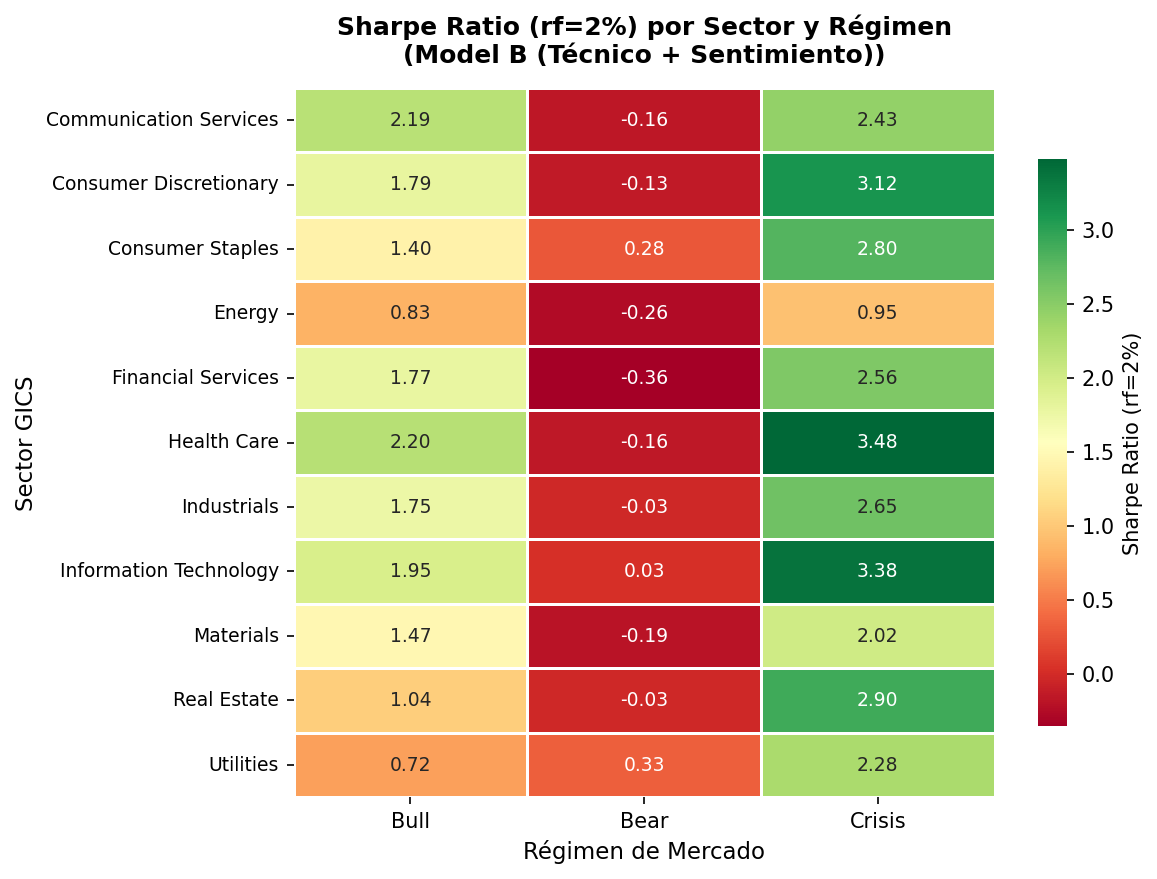
\includegraphics[width=0.85\textwidth]{figures/fig_heatmap_sharpe_modelB.png}
  \caption{Sharpe ratio by GICS sector and regime, Model B (\texttt{kmeans\_tech\_sent}).}
  \label{fig:heatmap-sharpe-modelB}
\end{figure}

\Cref{fig:heatmap-sharpe-modelB} shows that the \textbf{Bear} regime
produces a \emph{negative} Sharpe ratio for \textbf{10 of the 11 GICS
sectors} (all except \emph{Consumer Staples}, which remains marginally
positive at $0.28$), with the most negative values observed in
\emph{Financial Services} ($-0.36$), \emph{Energy} ($-0.26$),
\emph{Materials} ($-0.19$) and \emph{Real Estate} ($-0.19$). This is the
clearest evidence that the \emph{Bear} regime, as detected by Model B,
corresponds to a genuinely adverse environment across virtually the entire
equity market, not merely for the aggregate index. By contrast, the
\textbf{Crisis} regime shows the \emph{highest} Sharpe ratio for every
single sector, ranging from $0.95$ (\emph{Energy}) to as high as $3.48$
(\emph{Health Care}) and $3.38$ (\emph{Information Technology}). Averaged
across sectors, the mean regime Sharpe ratios for Model B are $1.56$
(Bull), $-0.06$ (Bear) and $2.60$ (Crisis) --- the same qualitative pattern
observed at the aggregate market level in \Cref{tab:market-kmeans}, now
confirmed to hold sector-by-sector.

\begin{figure}[H]
  \centering
  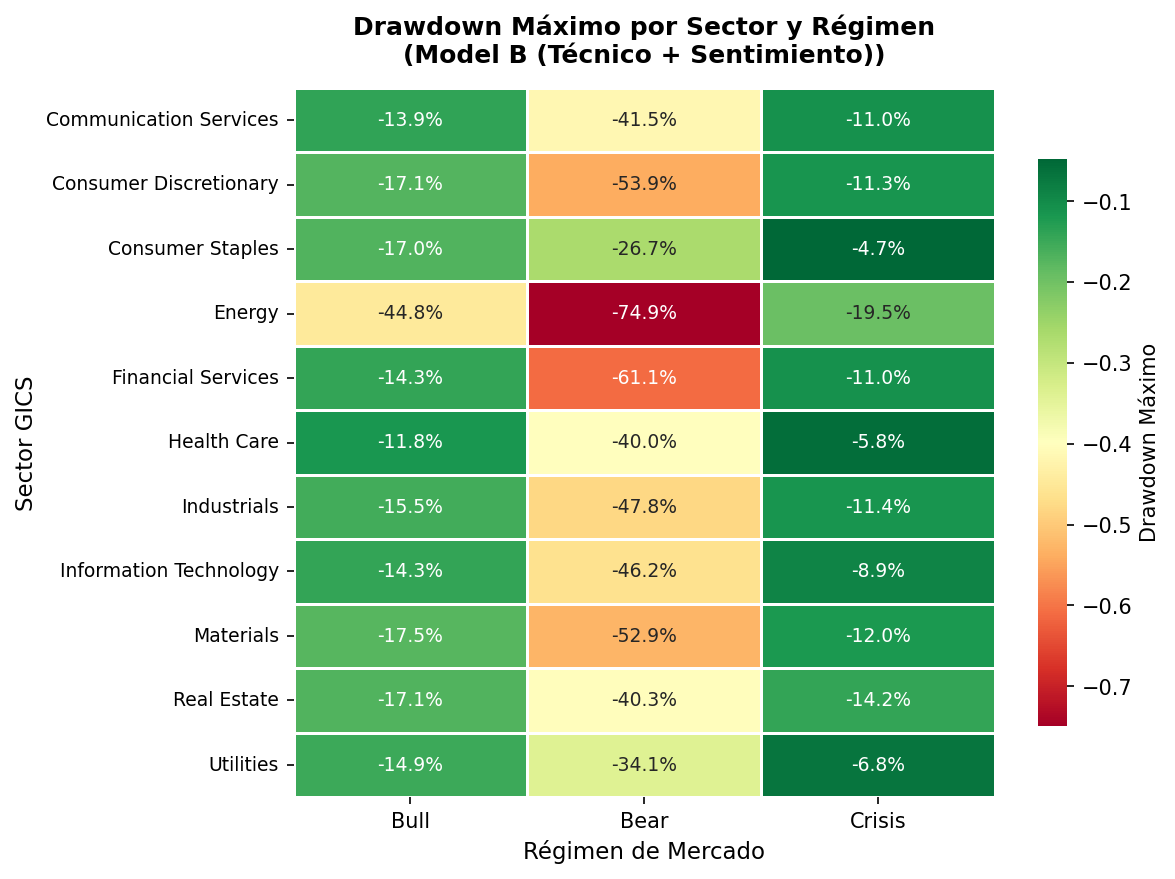
\includegraphics[width=0.85\textwidth]{figures/fig_heatmap_maxdd_modelB.png}
  \caption{Maximum (within-regime) drawdown by GICS sector and regime, Model B (\texttt{kmeans\_tech\_sent}).}
  \label{fig:heatmap-maxdd-modelB}
\end{figure}

\Cref{fig:heatmap-maxdd-modelB} shows that the single most severe
within-regime drawdown across the entire analysis occurs for
\textbf{\emph{Energy} in the \emph{Bear} regime}, at $-74.9\%$ --- more
than 20 percentage points worse than the next most severe combination
(\emph{Financial Services}/Bear at $-61.1\%$). Averaged across sectors,
the mean maximum drawdown by regime is $-18.0\%$ (Bull), $-47.2\%$ (Bear)
and $-10.6\%$ (Crisis): the \emph{Bear} regime is associated with
substantially deeper drawdowns than \emph{Crisis}, despite \emph{Crisis}
having higher \emph{point-in-time} volatility (\Cref{tab:centroids-modelB}).
This apparent paradox is resolved by recalling that \emph{Crisis} days are
characterized by \emph{both} large negative \emph{and} large positive
daily moves (high volatility with a strong rebound component, captured by
the elevated \texttt{mom126\_sp500} centroid), whereas \emph{Bear} days
tend to be more \emph{persistently} negative, allowing losses to compound
into deeper drawdowns even though individual daily moves are, on average,
less extreme.

\begin{figure}[H]
  \centering
  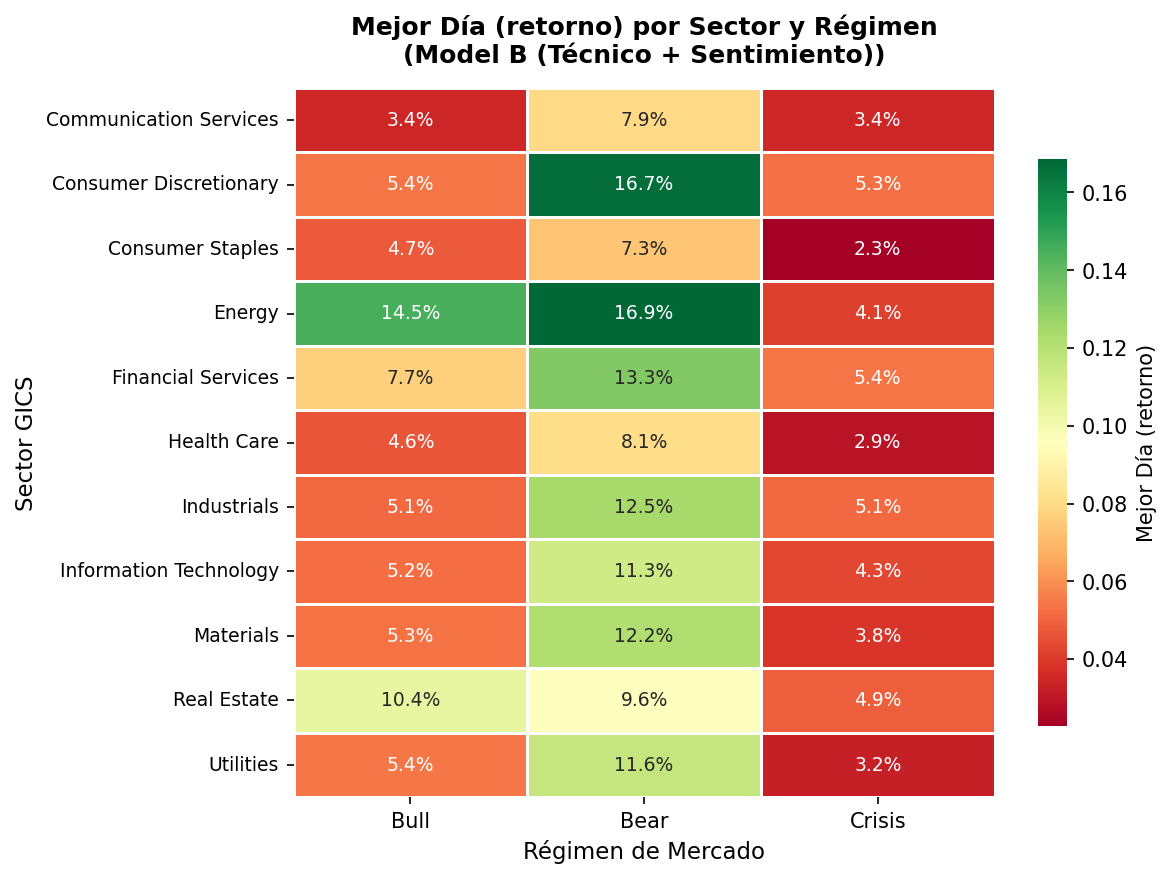
\includegraphics[width=0.85\textwidth]{figures/fig_heatmap_bestday_modelB.png}
  \caption{Best single-day return by GICS sector and regime, Model B (\texttt{kmeans\_tech\_sent}).}
  \label{fig:heatmap-bestday-modelB}
\end{figure}

\begin{figure}[H]
  \centering
  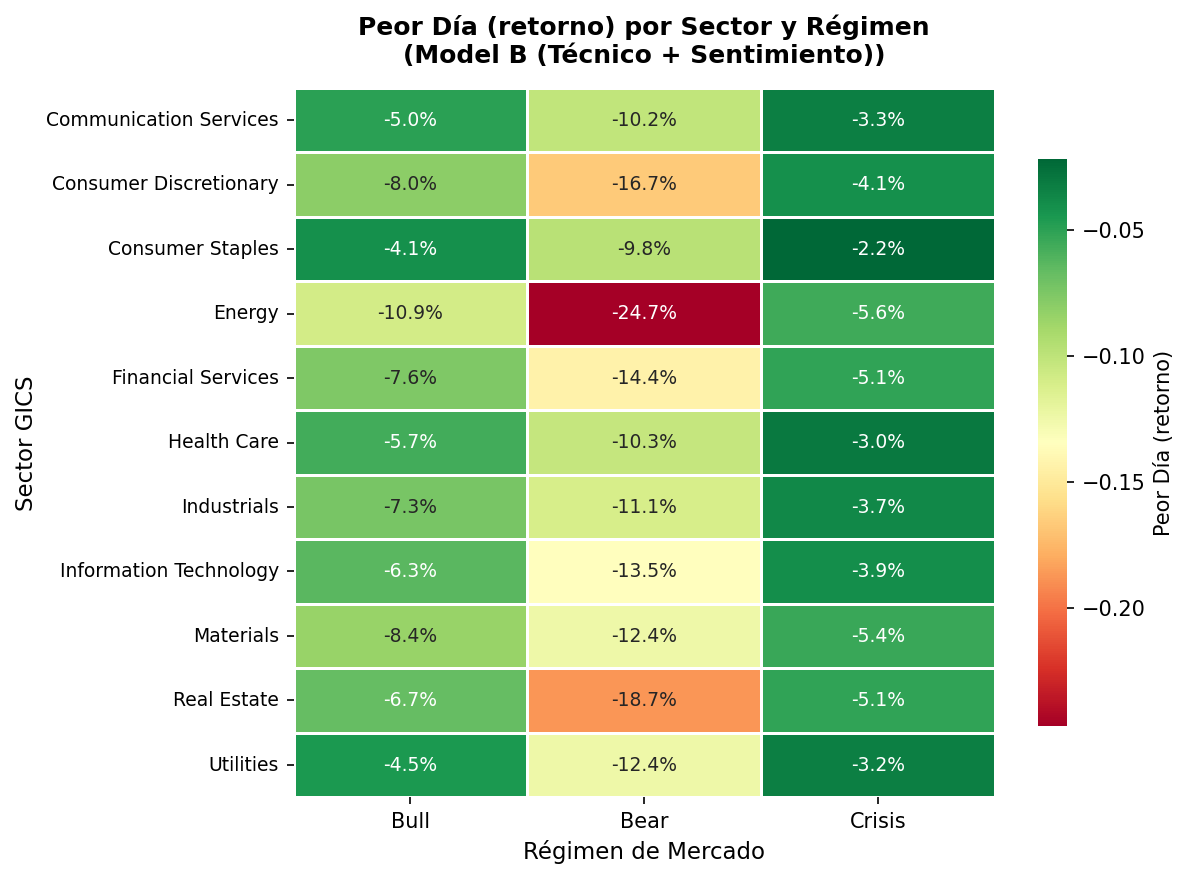
\includegraphics[width=0.85\textwidth]{figures/fig_heatmap_worstday_modelB.png}
  \caption{Worst single-day return by GICS sector and regime, Model B (\texttt{kmeans\_tech\_sent}).}
  \label{fig:heatmap-worstday-modelB}
\end{figure}

\Cref{fig:heatmap-bestday-modelB,fig:heatmap-worstday-modelB} reveal a
striking fact: the \textbf{single best day} ($+16.9\%$) \emph{and} the
\textbf{single worst day} ($-24.7\%$) of the \emph{entire dataset}, across
all sectors and all regimes, both occur for \textbf{\emph{Energy} in the
\emph{Bear} regime}. This confirms that, for Model B, the \emph{Bear}
regime --- rather than \emph{Crisis} --- is where the most extreme
single-day tail events are concentrated for the \emph{Energy} sector,
likely reflecting episodes such as the April 2020 negative oil-price
shock, which combined a severe and \emph{persistent} (Bear-like) downturn
in energy markets with extreme single-day volatility.

The corresponding Sharpe-ratio heatmaps for Models A and C are shown in
\Cref{fig:heatmap-sharpe-modelA,fig:heatmap-sharpe-modelC} for reference;
Model A shows a qualitatively similar but slightly less extreme pattern
than Model B (mean regime Sharpe ratios of $1.41$, $-0.07$ and $2.44$ for
Bull, Bear and Crisis respectively), while Model C is discussed separately
in \Cref{sec:results-modelC}.

\begin{figure}[H]
  \centering
  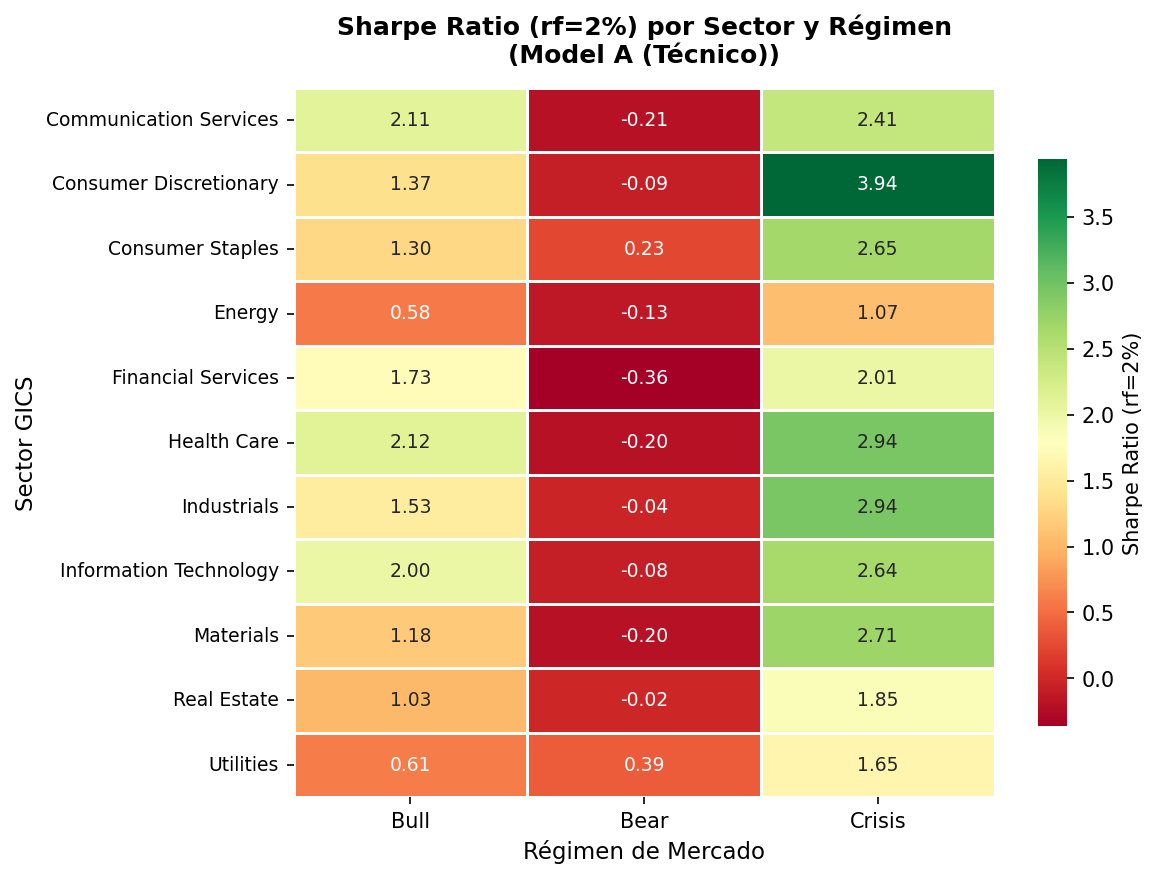
\includegraphics[width=0.85\textwidth]{figures/fig_heatmap_sharpe_modelA.png}
  \caption{Sharpe ratio by GICS sector and regime, Model A (\texttt{kmeans\_tech}).}
  \label{fig:heatmap-sharpe-modelA}
\end{figure}

\section{Model C: A Negative Result}
\label{sec:results-modelC}

Model C clusters days using \emph{exclusively} the 11 MA21-smoothed sector
sentiment features, with no technical (price-derived) information
whatsoever. \Cref{fig:heatmap-sharpe-modelC} shows the resulting Sharpe
ratio heatmap.

\begin{figure}[H]
  \centering
  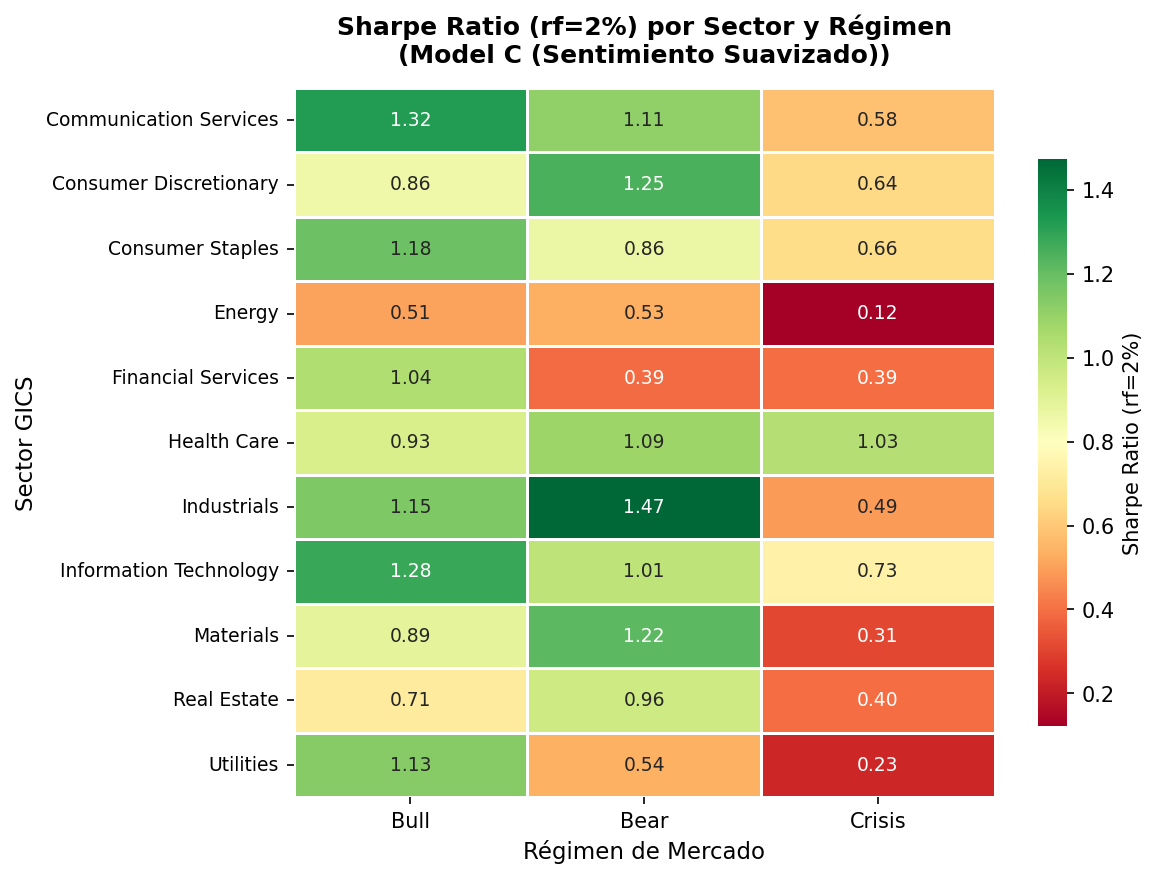
\includegraphics[width=0.85\textwidth]{figures/fig_heatmap_sharpe_modelC.png}
  \caption{Sharpe ratio by GICS sector and regime, Model C (\texttt{kmeans\_sent\_smooth}).}
  \label{fig:heatmap-sharpe-modelC}
\end{figure}

Two pieces of evidence jointly indicate that Model C fails to recover
regimes with a technical/economic profile comparable to Models A and B.

First, \textbf{the technical centroids of Model C's three clusters are
nearly indistinguishable} (\Cref{tab:centroids-modelC}). For example,
\texttt{MA50\_ratio\_sp500} ranges only from $1.0086$ to $1.0134$ across
Model C's clusters --- a spread of $0.0048$ --- compared to a spread of
$0.0653$ for Model A ($0.9739$ to $1.0392$) and $0.0608$ for Model B. The
\texttt{RSI\_sp500} centroids similarly range only from $54.4$ to $56.2$
for Model C, compared to $42.6$--$60.3$ for Model A.

\begin{table}[H]
\centering
\caption{Model C (smoothed sentiment only): centroids in the \emph{technical} feature space (for comparison with Models A and B), and cluster sizes.}
\label{tab:centroids-modelC}
\small
\begin{tabular}{lrrr}
\toprule
\textbf{Feature} & \textbf{Cluster 0} & \textbf{Cluster 1} & \textbf{Cluster 2} \\
\midrule
RSI\_sp500          & 54.86 & 54.44 & 56.18 \\
MA50\_ratio\_sp500  & 1.0086 & 1.0134 & 1.0109 \\
MA200\_ratio\_sp500 & 1.0274 & 1.0924 & 1.0496 \\
mom21\_sp500        & 0.0081 & 0.0063 & 0.0094 \\
mom126\_sp500       & 0.0379 & 0.1397 & 0.0683 \\
vol30d\_sp500       & 0.1532 & 0.1389 & 0.1260 \\
vol252d\_sp500      & 0.1633 & 0.2135 & 0.1402 \\
skew30d\_sp500      & $-$0.0460 & $-$0.3928 & $-$0.2998 \\
skew252d\_sp500     & $-$0.3193 & $-$0.3215 & $-$0.5746 \\
\midrule
\textbf{$n$ (days)}  & \textbf{534} & \textbf{172} & \textbf{426} \\
\bottomrule
\end{tabular}
\end{table}

Second, \textbf{the economic differentiation of Model C's regimes is much
weaker} than that of Models A and B. The mean Sharpe ratios across sectors
are $1.00$ (Bull), $0.95$ (Bear) and $0.51$ (Crisis) for Model C
(\Cref{tab:market-kmeans} reports the corresponding market-level figures
of $0.83$, $1.70$ and $-0.48$). Strikingly, Model C's ``Bear'' regime has
a Sharpe ratio \emph{higher} than its ``Bull'' regime at the market level
($1.70$ vs.\ $0.83$), the \emph{opposite} of what is observed for Models A
and B, and its ``Crisis'' regime --- which, at $45.7\%$ of all
sector-days, is by far the \emph{largest} regime under Model C (compared
to $5.4$--$10.1\%$ for Models A/B) --- has the \emph{lowest} mean Sharpe
ratio of the three. This inversion confirms that the regime labels
inherited from the $\{0,1,2\} \to \{\text{Bull},\text{Bear},\text{Crisis}\}$
mapping (\Cref{sec:meth-labeling}), while mechanically applied for
consistency with Models A and B, do not carry the same economic meaning
for Model C: the underlying \emph{partition itself} does not correspond to
the technical Bull/Bear/Crisis structure observed in Models A and B.

\Cref{fig:sharpe-comparativa} visualizes this contrast directly: the
market-level Sharpe ratios of clusters 0, 1 and 2 are plotted side by side
for \texttt{kmeans\_tech} (Model A), \texttt{kmeans\_tech\_sent} (Model B)
and \texttt{kmeans\_sent\_smooth} (Model C). Models A and B display the
same qualitative pattern --- two clusters with strongly positive Sharpe
ratios (around $+3.3$ to $+3.8$) and one with a strongly negative Sharpe
ratio (around $-3.1$) --- whereas Model C's three clusters all have Sharpe
ratios within a much narrower band ($-0.5$ to $+1.7$), with \emph{none}
reaching the magnitude of any cluster in Models A or B. This figure
provides a compact, side-by-side summary of the central negative result of
this section: smoothed-sentiment-only clustering produces regimes that are
economically far less differentiated than either technical-only or
technical+sentiment clustering.

\begin{figure}[H]
  \centering
  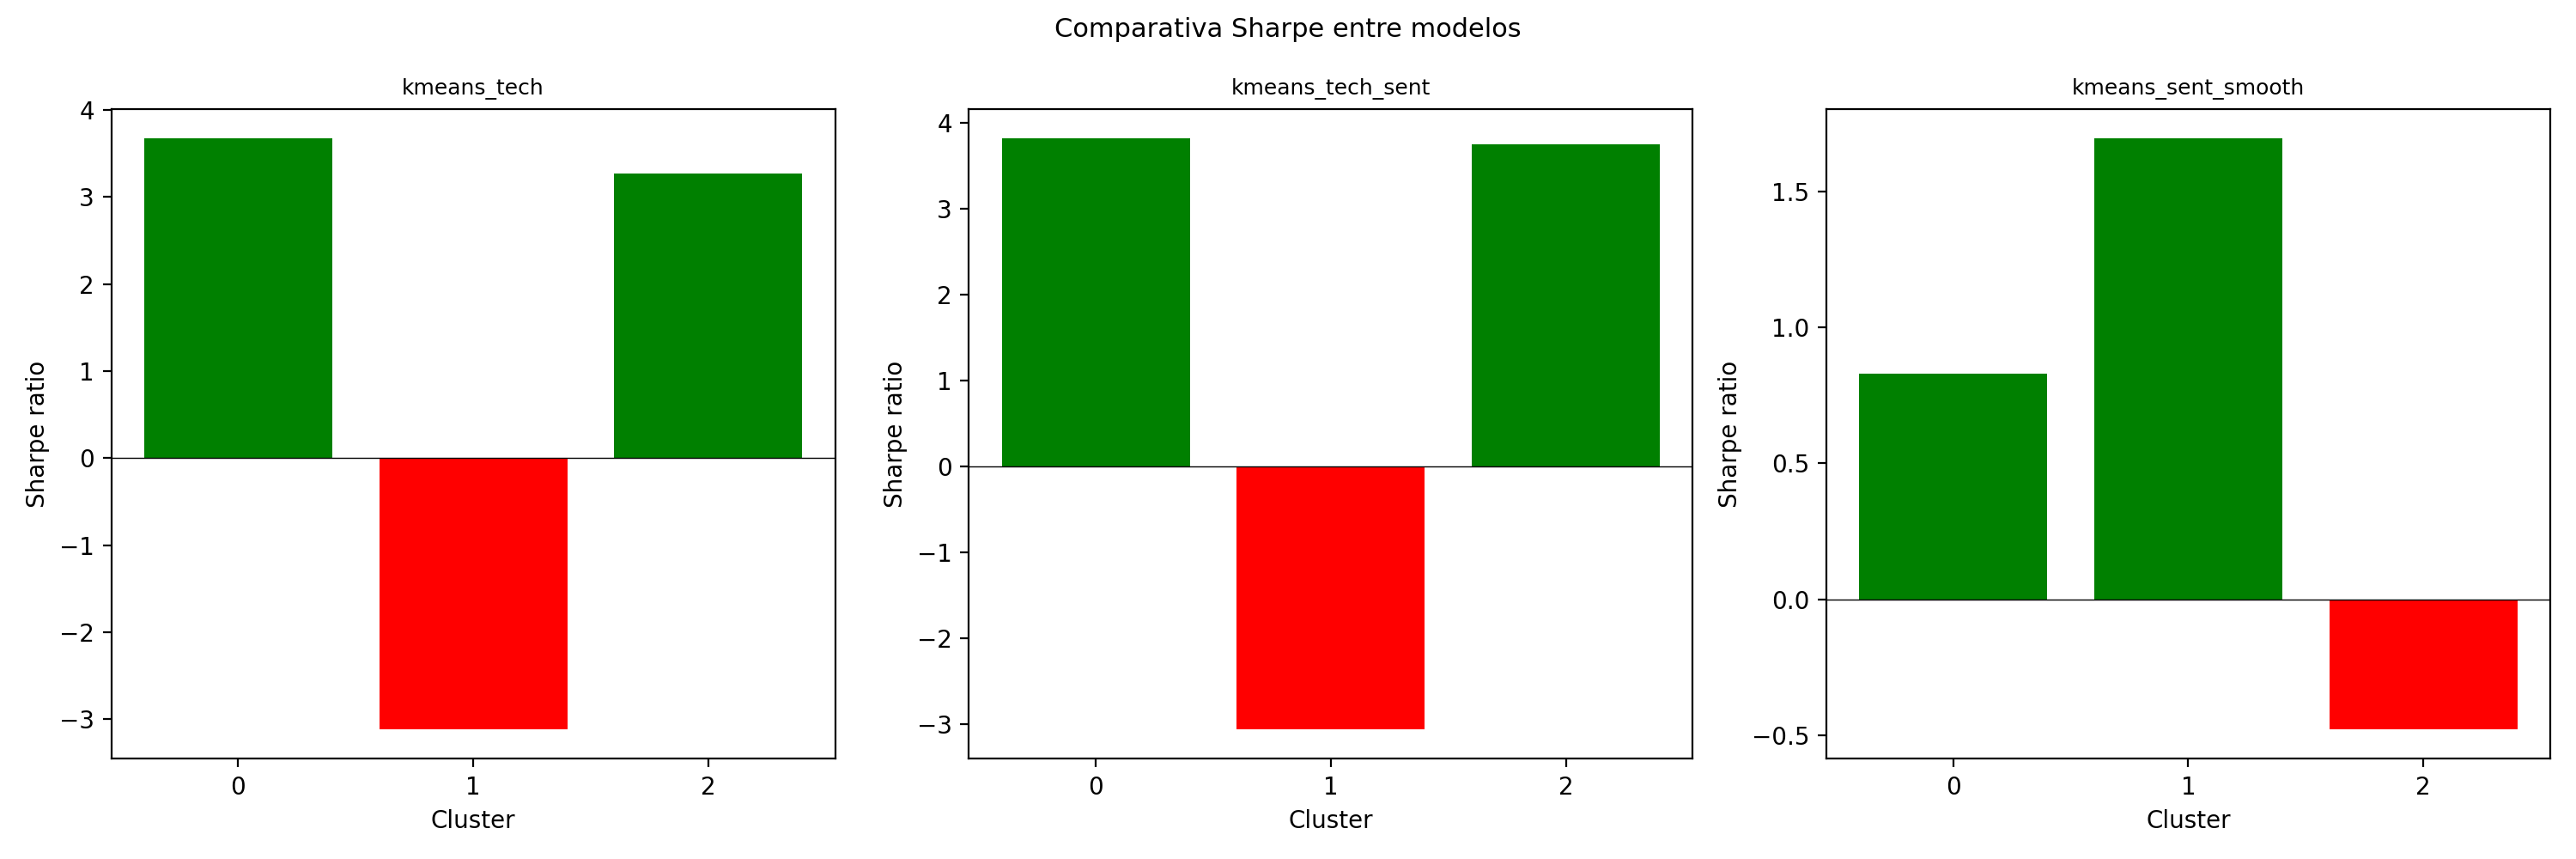
\includegraphics[width=\textwidth]{figures/fig_sharpe_comparativa.png}
  \caption{Market-level Sharpe ratio by cluster for Models A (\texttt{kmeans\_tech}), B (\texttt{kmeans\_tech\_sent}) and C (\texttt{kmeans\_sent\_smooth}). Green bars indicate a positive Sharpe ratio, red bars a negative Sharpe ratio.}
  \label{fig:sharpe-comparativa}
\end{figure}

Taken together, these results constitute a \textbf{meaningful negative
finding}: aggregated sector sentiment, even after MA21 smoothing
specifically designed to capture medium-term trends
(\Cref{sec:meth-smoothing}), does \emph{not}, on its own, recover a
partition of trading days that aligns with either the technical regime
structure or a monotonic economic (Sharpe ratio) ordering. This does not
imply that sentiment is uninformative --- Model B's results
(\Cref{sec:results-econ-sector}) and the feature-importance analysis
(\Cref{sec:results-importance}) show that sentiment-derived features,
particularly \texttt{sentiment\_std} columns, contribute meaningfully
\emph{when combined with} technical features. Rather, it indicates that
sentiment functions as a \emph{complement} to price information, not as a
\emph{substitute} for it, at least at the sector-aggregation and smoothing
granularity considered in this thesis.

\section{K-Means versus Gaussian HMM}
\label{sec:results-hmm}

\Cref{tab:market-hmm} (\Cref{sec:results-econ-overall}) reported the
market-level Sharpe ratios for the two Gaussian HMM variants:
\texttt{hmm\_tech} ($-0.63$ to $+1.54$) and \texttt{hmm\_tech\_sent}
($-0.25$ to $+1.25$). Comparing these ranges to the corresponding
\textit{K-Means} ranges --- $-3.12$ to $+3.68$ for Model A, and $-3.06$ to
$+3.82$ for Model B --- shows that the \textbf{spread of Sharpe ratios
across regimes/states produced by the HMM is roughly 4--5 times narrower
than that produced by K-Means}, for both the technical-only and
technical+sentiment feature sets.

This finding is consistent with the theoretical discussion in
\Cref{sec:soa-hmm}: the HMM's transition matrix imposes \emph{temporal
persistence} on the state sequence (a day is likely to remain in the same
state as the previous day, governed by the diagonal of the transition
matrix), which tends to produce states that are temporal
\emph{aggregates} of more homogeneous sub-periods. \textit{K-Means}, by
contrast, assigns each day independently to the cluster whose centroid it
is closest to in feature space, with no penalty for switching clusters
from one day to the next. As a result, \textit{K-Means} can isolate a
small number of \emph{extreme} days (e.g., Model A's and B's
\emph{Crisis} regime, $n=70$, 6.2\% of the sample) into their own cluster,
producing a centroid --- and therefore an economic profile --- that is
sharply different from the other two clusters. The HMM's states, being
constrained by transition dynamics, instead tend to blend such extreme
days together with the surrounding, less extreme days of the same
\emph{episode}, producing milder, more ``averaged'' state-level
statistics.

From a practical standpoint, this represents a genuine
\textbf{trade-off} rather than a simple ranking of ``better'' versus
``worse'' models. \textit{K-Means}'s sharper regimes are more useful for
\emph{characterizing} what an extreme regime looks like economically
(as in \Cref{sec:results-econ-sector}), since its \emph{Crisis} cluster is
not diluted by adjacent, more moderate days. The HMM's smoother regimes,
on the other hand, may be more directly useful for \emph{real-time
monitoring} or \emph{trading} applications, where a regime indicator that
switches state on every isolated extreme day (as \textit{K-Means} labels
can, since they carry no explicit persistence constraint) would generate
excessive turnover. \Cref{fig:hmm-states-modelA,fig:hmm-states-modelB}
(\Cref{sec:results-regimes}) illustrate this: the HMM states visibly
persist over multi-week to multi-month spans, in line with the
\texttt{vol30d\_sp500} dynamics, whereas the \textit{K-Means}-based regime
shading in \Cref{fig:sp500-regimes-modelA,fig:sp500-regimes-modelB} shows a
\emph{Crisis} regime confined to brief, sharply-defined episodes.

\section{Summary of Key Findings}
\label{sec:results-summary}

The results presented in this chapter can be summarized in five key
findings:

\begin{enumerate}
  \item \textbf{Technical indicators remain the strongest structural
  discriminator}, both in terms of silhouette coefficient in the common
  PCA space (Model A: 0.1928 vs.\ Model B: 0.1778 vs.\ Model C: 0.1623,
  \Cref{tab:silhouette-comparison}) and in terms of ANOVA feature
  importance (the top 6 features for Model B are all technical,
  \Cref{tab:feature-importance}).

  \item \textbf{Sentiment-augmented clustering (Model B) sharpens economic
  differentiation relative to the technical-only baseline (Model A)},
  particularly for the \emph{Bull} and \emph{Crisis} regimes (market-level
  Sharpe of $3.82$ and $3.75$ for Model B vs.\ $3.68$ and $3.28$ for Model
  A), while the \emph{Bear} regime becomes negative across nearly all
  sectors (10 of 11) under Model B.

  \item \textbf{The \emph{Bear} regime is the only regime with negative
  Sharpe ratios at both the market and (almost universally) the sector
  level}, while the \emph{Crisis} regime --- despite having the highest
  volatility --- has the \emph{highest} Sharpe ratios across all sectors,
  reflecting its association with sharp V-shaped recoveries (2009, 2020)
  rather than sustained losses.

  \item \textbf{The \emph{Energy} sector in the \emph{Bear} regime is the
  single most extreme combination in the dataset}: it has the worst
  maximum drawdown ($-74.9\%$) of any sector/regime combination, and
  contains both the best ($+16.9\%$) and the worst ($-24.7\%$) single-day
  returns of the entire sample.

  \item \textbf{Sentiment alone (Model C) is not a viable substitute for
  technical indicators}: its cluster centroids are nearly
  indistinguishable in technical-feature space, and its inherited
  Bull/Bear/Crisis labels do not preserve a monotonic Sharpe-ratio
  ordering. \textbf{The Gaussian HMM produces qualitatively similar but
  quantitatively much milder regimes than K-Means} (Sharpe ratio ranges
  roughly 4--5 times narrower), reflecting the trade-off between temporal
  persistence and sharp economic differentiation.
\end{enumerate}

These findings are discussed further, together with their limitations and
implications for future work, in \Cref{ch:conclusions}.
